%%%%%%%%%%%%%%%%%%%%%%%%%%%%%%%%%%%%%%%%%%%%%%%%%%%%%%%%%%%%%%%%%%%%%%%%%%%%%%%%
% Document Class %%%%%%%%%%%%%%%%%%%%%%%%%%%%%%%%%%%%%%%%%%%%%%%%%%%%%%%%%%%%%%%
%%%%%%%%%%%%%%%%%%%%%%%%%%%%%%%%%%%%%%%%%%%%%%%%%%%%%%%%%%%%%%%%%%%%%%%%%%%%%%%%
\documentclass[letterpaper]{article}

%%%%%%%%%%%%%%%%%%%%%%%%%%%%%%%%%%%%%%%%%%%%%%%%%%%%%%%%%%%%%%%%%%%%%%%%%%%%%%%%
%Encoding & Language %%%%%%%%%%%%%%%%%%%%%%%%%%%%%%%%%%%%%%%%%%%%%%%%%%%%%%%%%%%
%%%%%%%%%%%%%%%%%%%%%%%%%%%%%%%%%%%%%%%%%%%%%%%%%%%%%%%%%%%%%%%%%%%%%%%%%%%%%%%%
\usepackage{float} % to supress floating of tables
%\usepackage[utf8]{inputenc}
\usepackage[T1]{fontenc}
\usepackage[latin1]{inputenc}
\usepackage{float}

\usepackage{booktabs}


\synctex=1


%%%%%%%%%%%%%%%%%%%%%%%%%%%%%%%%%%%%%%%%%%%%%%%%%%%%%%%%%%%%%%%%%%%%%%%%%%%%%%%%
% Fonts %%%%%%%%%%%%%%%%%%%%%%%%%%%%%%%%%%%%%%%%%%%%%%%%%%%%%%%%%%%%%%%%%%%%%%%%
%%%%%%%%%%%%%%%%%%%%%%%%%%%%%%%%%%%%%%%%%%%%%%%%%%%%%%%%%%%%%%%%%%%%%%%%%%%%%%%%

%\Usepackage{mathptmx}
\renewcommand{\familydefault}{\sfdefault}
%\usepackage{helvet}
%\setmainfont[Ligatures=TeX]{HelveticaLight.ttf}
%\usepackage{lmodern}
%\usepackage{amsthm}
%\usepackage{amsfonts}
%\usepackage{amsmath}
%\usepackage[type1]{biolinum}
%\usepackage[sc,osf]{mathpazo}
%\usepackage[scaled=0.95]{inconsolata}
%\usepackage[euler-digits,small]{eulervm}

%%%%%%%%%%%%%%%%%%%%%%%%%%%%%%%%%%%%%%%%%%%%%%%%%%%%%%%%%%%%%%%%%%%%%%%%%%%%%%%%
%%%%%%%%%%%%%%%%%%%%%%%%%%%%%%%%%%%%%%%%%%%%%%%%%%%%%%%%%%%%%%%%%%%%%%%%%%%%%%%%
%%%%%%%%%%%%%%%%%%%%%%%%%%%%%%%%%%%%%%%%%%%%%%%%%%%%%%%%%%%%%%%%%%%%%%%%%%%%%%%%

%\usepackage{fancyvrb}
%\usepackage{geometry}
%\usepackage{float}
%\usepackage{graphicx}
%\usepackage{comment}
%\usepackage{multirow}
%\usepackage{latexsym}
%\usepackage{tabularx}
%\usepackage{longtable} % tables spanning multiple pages
%\usepackage{ltxtable} %tabularx tables spanning multiple pages
\usepackage{verbatim}
\usepackage{parskip}
\usepackage{pdfpages}
\usepackage{url}
\usepackage[colorlinks=false,linkcolor=black,hidelinks,urlcolor=blue,citecolor=black,bookmarks=true]{hyperref}
%\usepackage{array} % For centered fixed width columns
\usepackage{fullpage}

%%%%%%%%%%%%%%%%%%%%%%%%%%%%%%%%%%%%%%%%%%%%%%%%%%%%%%%%%%%%%%%%%%%%%%%%%%%%%%%%
% Auctex Preview %%%%%%%%%%%%%%%%%%%%%%%%%%%%%%%%%%%%%%%%%%%%%%%%%%%%%%%%%%%%%%%
%%%%%%%%%%%%%%%%%%%%%%%%%%%%%%%%%%%%%%%%%%%%%%%%%%%%%%%%%%%%%%%%%%%%%%%%%%%%%%%%

%\usepackage[auctex,active,psfixbb,showlabels,sections,floats,textmath,graphics,displaymath]{preview}

%%%%%%%%%%%%%%%%%%%%%%%%%%%%%%%%%%%%%%%%%%%%%%%%%%%%%%%%%%%%%%%%%%%%%%%%%%%%%%%%
%%%%%%%%%%%%%%%%%%%%%%%%%%%%%%%%%%%%%%%%%%%%%%%%%%%%%%%%%%%%%%%%%%%%%%%%%%%%%%%%
%%%%%%%%%%%%%%%%%%%%%%%%%%%%%%%%%%%%%%%%%%%%%%%%%%%%%%%%%%%%%%%%%%%%%%%%%%%%%%%%

%\linespread{1.025}

\newcommand*\inverse[1]{\bar{#1}}

%%%%%%%%%%%%%%%%%%%%%%%%%%%%%%%%%%%%%%%%%%%%%%%%%%%%%%%%%%%%%%%%%%%%%%%%%%%%%%%%
%%%%%%%%%%%%%%%%%%%%%%%%%%%%%%%%%%%%%%%%%%%%%%%%%%%%%%%%%%%%%%%%%%%%%%%%%%%%%%%%
\renewcommand{\sectionautorefname}{\S}
\renewcommand{\subsectionautorefname}{\S}
\renewcommand{\subsubsectionautorefname}{\S}

%%%%%%%%%%%%%%%%%%%%%%%%%%%%%%%%%%%%%%%%%%%%%%%%%%%%%%%%%%%%%%%%%%%%%%%%%%%%%%%%
% Adds an untypeset section (i.e. it will appear in index but the heading won't be print)
%%%%%%%%%%%%%%%%%%%%%%%%%%%%%%%%%%%%%%%%%%%%%%%%%%%%%%%%%%%%%%%%%%%%%%%%%%%%%%%%
\newcommand{\nosection}[1]{%
    \refstepcounter{section}%
    \addcontentsline{toc}{section}{\protect\numberline{\thesection}#1}%
\markright{#1}}

\newcommand{\nosubsection}[1]{%
    \refstepcounter{section}%
    \addcontentsline{toc}{section}{\protect\numberline{\thesubsection}#1}%
\markright{#1}}


%\newcolumntype{x}[1]{>{\centering\arraybackslash\hspace{0pt}}p{#1}}
%\newcolumntype{L}[1]{>{\raggedright\let\newline\\\arraybackslash\hspace{0pt}}m{#1}}
%\newcolumntype{C}[1]{>{\centering\let\newline\\\arraybackslash\hspace{0pt}}m{#1}}
%\newcolumntype{R}[1]{>{\raggedleft\let\newline\\\arraybackslash\hspace{0pt}}m{#1}}


\title{LCT Comparator ASIC \\ Description and Testing Information}
\author{UCLA High Energy Physics}

\begin{document}

\maketitle

\tableofcontents

\section{Summary}

The LCT-Comparator is a custom ASIC designed to generate fast trigger information for the CMS muon endcap's cathode strip chambers. It is responsible for producing digital ``half-strip'' resolution trigger information by comparing the relative amplitudes of the full-strip analog signals that are coming from the chamber's cathode strips.

The chip operates by using an array of analog comparators to perform two primary functions:

\begin{enumerate}
    \item Determine whether the input signals are over a set threshold
    \item Compare neighboring channels to guess the location of charge deposition to half-strip resolution.
\end{enumerate}

Each IC handles inputs from 16 primary channels, but has additional analog inputs (one on each side) to connect to neighboring channels to ensure continuity across chips.  Each channel consists of a roughly 3.5 gain ac-coupled amplifier followed by an array of three comparators and a section of logic which digitizes and compresses the comparator half-strip.

To reduce the number of output conductors required, the outputs are encoded into a serialized three-bit sequence which is termed a triad. Thus, the 16 primary inputs are encoded on 8 ``di-strip'' output pins, which generate a three-bit serialized output sequence which encodes the half-strip position of the trigger. Each di-strip encodes the hits on two neighboring strips, or 4 neighboring half-strips.

The chip itself is a full ASIC integrated circuit fabricated with a 0.7$\mu$m nwell technology originating from Alcatel-Mietec in Belgium. The technology was sold by Alcatel-Mietec and both the process and IP now belongs to the American firm ON-Semiconductor. The foundry remains in Belgium, and small batch orders can still be produced through the same organization that arranged for the original fabrication, Europractice/IMEC (\url{http://www.europractice-ic.com/}). It is encapsulated into a standard TQFP-64 package.

\section{Chip Description}

To understand the comparator chip, it is useful to have some background on the problem that it is trying to solve:

We have a particle detector (specifically, a cathode strip chamber or CSC, which is just our brand-name for a multi-wire proportional counter or MWPC). The chamber has six layers of cathode strips and 6 layers of anode wires which run roughly either at a 29 degree angle to eachother (for ME1/1) or roughly perpendicular (all other stations).

Together, the cathode strips and anode wires provide an orthogonal coordinate system that allows for three-dimensional tracking of the passage of particles through the chamber.

The ionization medium inside the chamber is a high gain gas mixture composed of Ar/CO${_2}$/CF$_{4}$. When a charged particle passes through a chamber, it ionizes the gas and liberates a small number primary electronics.

Due to the high voltage between the anode wires and cathode strips (on the order of 3000--4000V), the primary electrons accelerate toward the anode wires. As secondary electrons are liberated, they too will accelerate toward the anode wires and liberate additional electrons. This produces a large charge multiplication, allowing the small number of initial ionizing electrons to be detected and read-out with relative ease. The gain of the process is on the order of several thousand, depending on the chamber geometry and voltage.

The signal received on the cathode strips comes from two sources:

Due to simple geometry, a small capacitive coupling exists between the anode wire and cathode strips, which causing a small mirrored signal to appear on the strips. A much slower drifting of ions (produced when electrons were liberated from neutral molecules), then takes places, which causes a much larger, slow signal to appear on the cathode strips. The source of the signal can best be thought of as an image charge induced on the strips from the free ions reamining in the gas. The signal will dissipate as the ions recombine with electrons.

The amplitude of thsignal is proportional to the amount of ionized charge, as well as the proximity of the path of traversal to the strip.  Typically the passage of a charged particle induces a distribution of charge on five neighboring strips, which can be seen diagrammatically in Fig.~\ref{fig:charge-distribution}. The shape of the charge can be mathematically modeled by a Gatti distribution (\url{www.physics.ohio-state.edu/~durkin/talks/gattiwidth.pdf}).

\small
\begin{figure}[H]
\begin{center}
\begin{minipage}{12cm}
\begin{verbatim}

                        +----+
                        |    |
                        |    |
                   +----+    |
                   |    |    |                    ^
                   |    |    |                    |
                   |    |    +----+               | Magnitude of
                   |    |    |    |               | induced charge
                   |    |    |    |               | on the strips (Q).
              +----+    |    |    |               |
Thresh (Vth)  |    |    |    |    +----+          |
------------  |    |    |    |    |    |          |
--------------+----+----+----+----+----+--------- |
Strips ->      n-2  n-1   n    n+1  n+2
\end{verbatim}
\end{minipage}
\end{center}
\caption{Cathode strip charge distribution: we can intuitively guess that the path of the particle would have passed closest to the left-side of strip n.}\label{fig:charge-distribution}
\end{figure}
\normalsize

The purpose of the comparator is to perform the fast identification of the center of the charge distribution to a ``half-strip'' accuracy. By comparing the relative amplitudes of pulses on neighboring strips, we are able to interpolate the half-strip location of the hit. For instance, in Figure~\ref{fig:charge-distribution} it can be easily seen that the particle would have passed through the left-half of strip n, based on the fact that n-1 > n+1.

To achieve this function, the LCT comparator ASIC consists of three basic parts:
\begin{enumerate}
    \item An array of 18 amplifiers which provide gain to the input signals (c.f. \autoref{sec:ac-amplifier})
    \item An analog comparator network that produces binary amplitude comparisons (c.f. \autoref{sec:comparator-array})
    \item A digital part that finds pulse peaks to half-strip accuracy and encodes the information into a compressed format to reduce the number of digital IOs. (c.f. \autoref{sec:triad-logic})
\end{enumerate}

\begin{figure}[H]
\centering
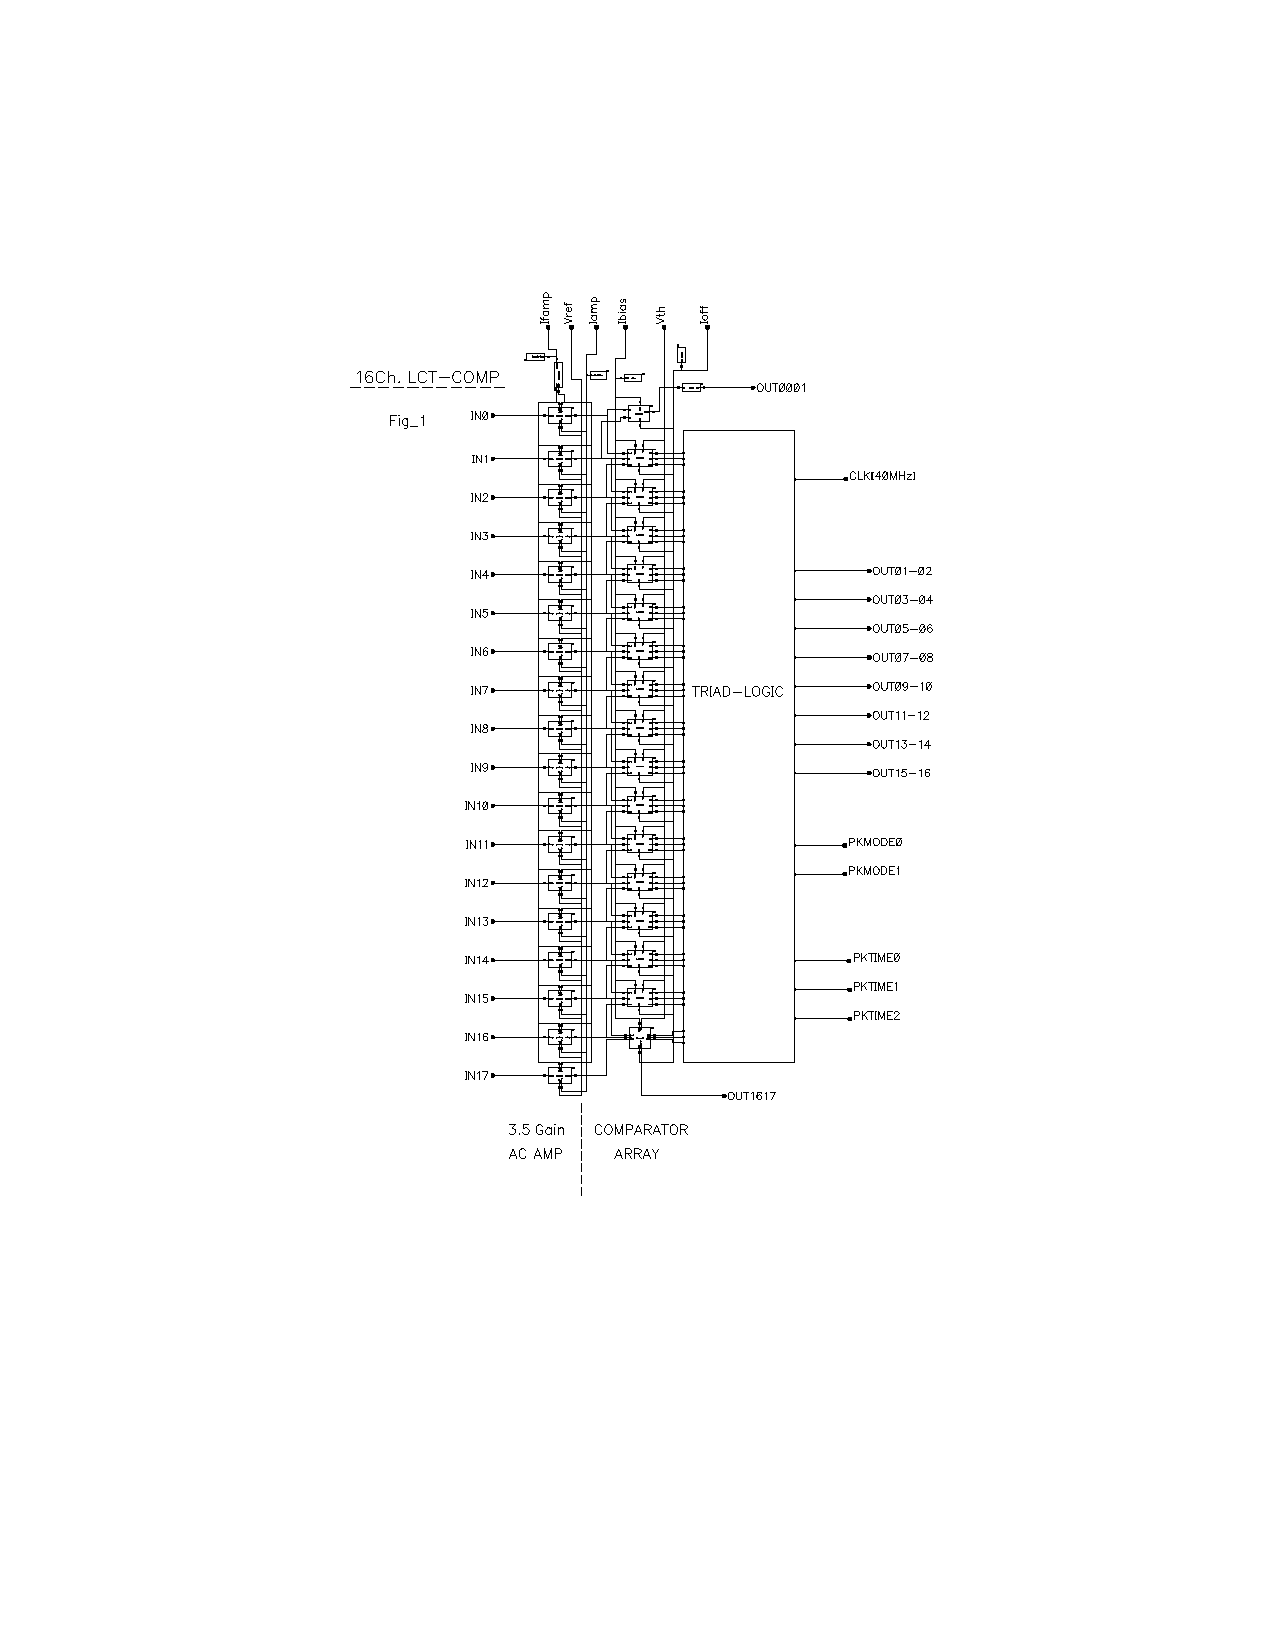
\includegraphics[keepaspectratio=true, width=1.1 \textwidth]{Images/amplifier_comparator_array_3.pdf}
\caption{Schematic diagram of the LCT-Comparator chip.}
\end{figure}

\subsection{AC Amplifier}\label{sec:ac-amplifier}

There are 16 analog cathode strip signals corresponding to each comparator ASIC.
The LCT-Comparator chip spends its life on a (D)CFEB---the (Digital) Cathode Front-end Board. Each (D)CFEB handles 16 cathode strips on each of 6 layers of CSC. The strips themselves are connected to The OSU produced "Buckeye" shaper/amplifier asic, which amplifies the pulse and shapes it into a predictably modeled semi-Gaussian waveform with peaking time around 100--150 ns.  The outputs from the buckeye chip are AC coupled to the 16 analog inputs of the comparator, with a voltage pull-up biasing the signals to a positive voltage reference. The pulses are of negative polarity.

The AC amplifier has an AC gain of approximately 3.5 and a DC gain of 0. It is made of an Operational Transconductance Amplifier with a capacitive element (see Fig.~\ref{fig:ac-amplifier}) in the feedback and also an OTA to stabilize the output offset compare to a reference level.

The input can accept DC variations of $\pm$100 mV without measurable change at the output, and the output rise time is 50 ns.

An AC-coupling capacitor has to be put as well as a resistor on the input of the LCT-COMP, connected to the $V_{REF}$ voltage (see schematic). Note: on the CFEB/DCFEB the value of the coupling capacitor is 0.001$\mu$F, with a pullup resistor of 4.7k to approximately 3.58V bias voltage.

\begin{figure}[H]
\label{fig:ac-amplifier}
\centering
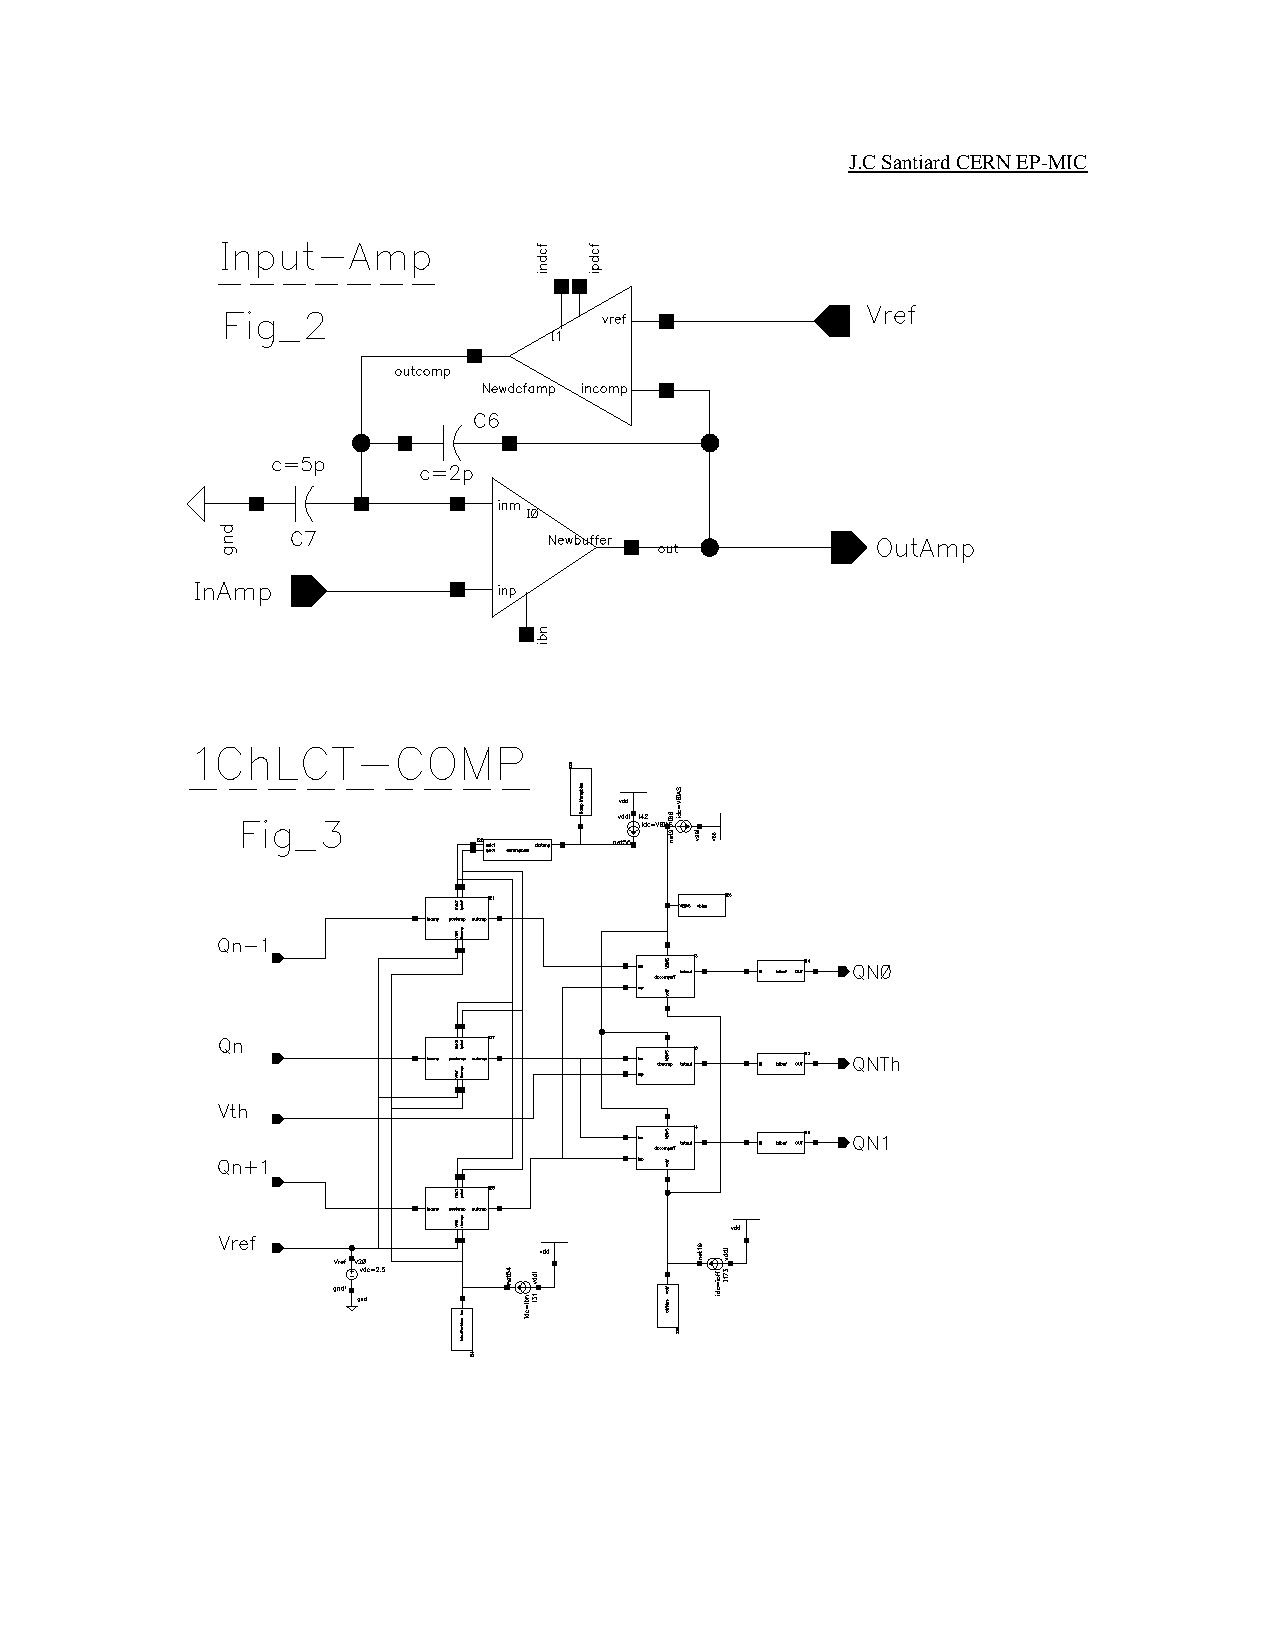
\includegraphics[keepaspectratio=true, width=1.0 \textwidth]{Images/ac-amplifier_and_comparator.pdf}
\caption{Schematic diagram of AC Input Amplifier (top) and a single channel's comparator array.}
\end{figure}

\subsection{Comparator Array}\label{sec:comparator-array}

Besides the 16 primary analog inputs (channels 1 to 16), there are separate inputs in channels 0 and 17 which are designed to connect to the previous and next comparator ASICs on the chamber, respectively. This is achieved by interconnects between neighboring CFEBs, which provide analog copies of their first and last outputs to the neighboring left and right boards, ensuring that there is complete continuity across an entire chamber.

There are 3 comparators per channel (1 to 16), but only one in the channels 0 and 17, for a total of 51 comparators in each chip.

Three channels [Fig. 3] are always involved in the comparison process: channel Q$_n$ is compare to a threshold and compare to channel Q$_{n+1}$ while channel Q$_{n-1}$ is compare to channel Q$_{n+1}$. The threshold is common to the 16 channels and adjustable through an outside pin. The offset of the other comparators can be adjusted as well to avoid oscillations.  To find the center of a charge distribution to a half-strip accuracy, the following algorithm is applied:

For a strip n:

\begin{enumerate}
    \item  Check if $Q_n > V_{th}$
    \item  Check if $Q_{n+1} > Q_{n-1}$
    \item  Check if $Q_{n+1} > Q_{n}$
\end{enumerate}

If all three conditions are met, then the selected half-strip is the ``left half strip of n''.  If (1.) and (3.) are true and (2.) is false, then the right half-strip is the ``right half-strip of n''.

\begin{figure}[H]
\centering 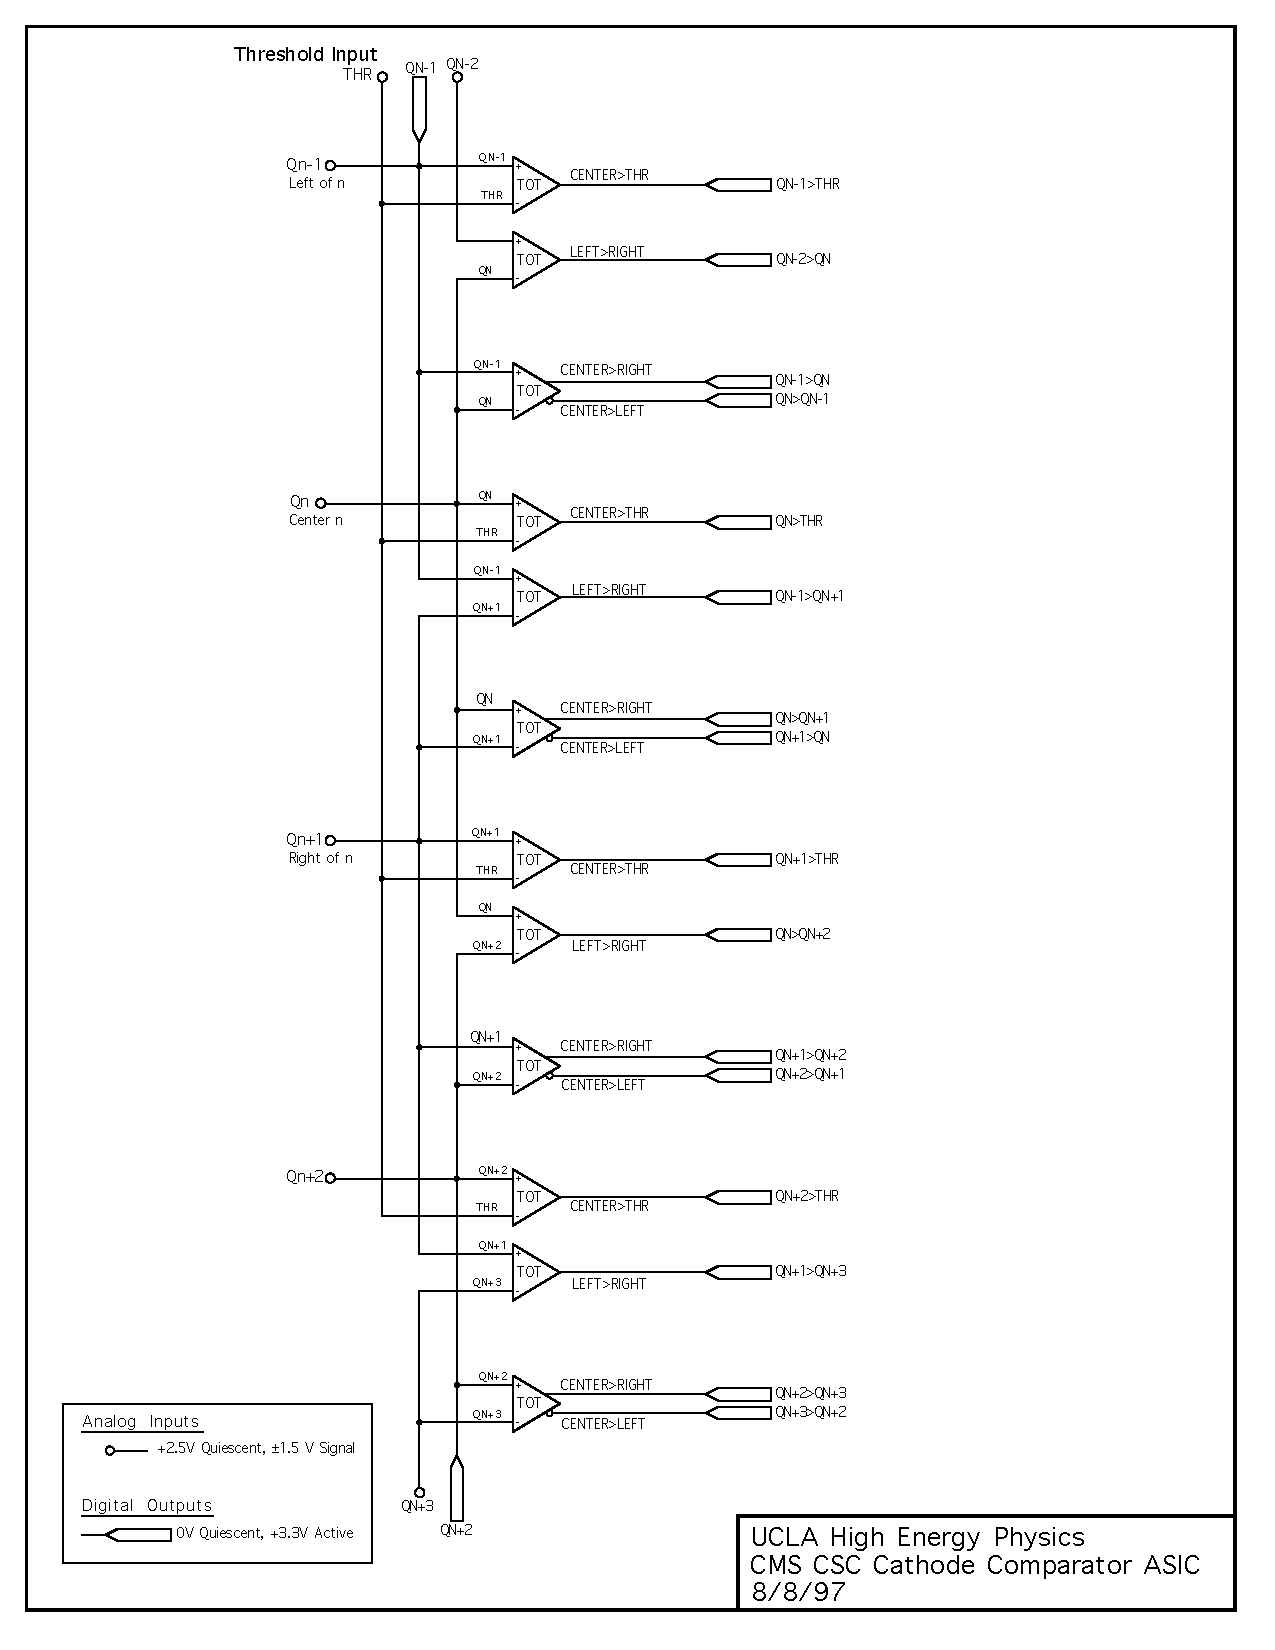
\includegraphics[keepaspectratio=true, width=0.9 \textwidth]{Images/synccompnodigital.pdf}
\caption{Schematic diagram of the LCT-Comparator analog amplifier and comparator arrays.}
\end{figure}

\subsection{Triad Logic}\label{sec:triad-logic}

The triad logic accepts the results of the comparisons done by the comparator array and uses them to identify the half-strip hit and send out the result in the following format:

There is one output pin for two strips (herein called a distrip). The output is a time sequence of three bits, with each bit coming after the next at the next clock cycle (CLK = 40 MHz / 25ns):

\begin{enumerate}
    \item If the first bit of the triad is asserted, it means that the distrip was hit (i.e.\ that one of the two strips that makes up the distrip was hit).
    \item If the second bit is 0, then it means that the first of the two strips was hit; if it is 1, then the second of the two strips was hit.
    \item If the third bit is 0, then it means that the first half strip (i.e.\ the left half strip) of the hit strip was hit; else, the second half strip (i.e.\ right half-strip) was hit.
\end{enumerate}

Or, more explicitly, we can decode the triad sequence as follows:

\renewcommand{\arraystretch}{1.2}
\begin{table}[H]
\begin{center}
\begin{tabular}{c l}
    \textbf{Triad [3:0]} & \textbf{Meaning} \\
    \midrule
    0XX & No Hit \\
    100 & Hit on 1st strip, left half-strip\\
    101 & Hit on 1st strip, right half-strip\\
    110 & Hit on 2nd strip, left half-strip \\
    111 & Hit on 2nd strip, right half-strip \\
\end{tabular}
\end{center}
\end{table}

\subsection{Ground}

\subsection{AVDD}

+5V analog supply. Should be as low noise as possible, with good ceramic decoupling capacitors (0.1 $\mu$F) placed close to each pin.

\subsection{DVDD}


DVDD0: 5V or +3.3V supply for the digital logic and 40MHz clock. For bypassing, use good ceramic decoupling capacitors (0.1 $\mu$F) placed close to each pin.

DVDD2: This supply feeds the output buffers, OUT0102 to OUT1516, it can be either +5V or +3.3V. Ceramic decoupling capcitors should be used, as before.

\subsection{Threshold Voltage}

Threshold of the comparator array. It has to be negative compared to the $V_{REF}$. Pin should be bypassed with the usual decoupling. Note that, due to the 3.5x gain of the AC amplifier, the threshold seen at the comparator inputs will be 1/3.5 the threshold applied to the pins. That is, for example, a $V_{TH}=50 mV$ requires a pulse of amplitude $>14.3$ mV to trigger.

\subsection{Bias Currents}

Four bias currents must be supplied to the comparator:

\begin{itemize}
    \item $I_{BIAS}$ Bias current of ca. 20 $\mu$A must be supplied to this pin, e.g. through a 130k resistor to $AV_{DD}$, with a 0.1 $\mu$F bypass capacitor.
    \item $I_{OFF}$  Bias current of ca. 2 $\mu$A must be supplied to this pin, e.g. through a 510k resistor to $AV_{DD}$, with a 0.1 $\mu$F bypass capacitor.  The offset current provides a programmable offset to the L>R comparator for each channel. Setting this offset prevents oscillations in the case of equal charge sharing between left and right half-strips.
    \item $I_{FAMP}$   Bias current of ca. 10 $\mu$A must be supplied to this pin, e.g. through a 390k resistor to $AV_{DD}$, with a 0.1 $\mu$F bypass capacitor.
    \item $I_{AMP}$    Bias current of ca. 80 $\mu$A must be supplied to this pin, e.g. through a 75k resistor to $AV_{DD}$, with a 0.1 $\mu$F bypass capacitor.

\end{itemize}

\subsubsection{ibias}
\subsubsection{ioff}
\subsubsection{ifamp}
\subsubsection{iamp}

\subsubsection{Reference Voltage}

$V_{REF}$ has to be built with a precise and stable reference voltage.  Normally no current is sunk or sourced from the different associated nodes. Good full decoupling. Note, on the CFEB/DCFEB the reference voltage is set to 3.59V.

\subsection{Neighboring Comparator Outputs}

\subsubsection{OUT0001}
        OUT0001 Provides comparator result $Q_{0}<Q_{1}$, i.e. that the first input on this CFEB is greater than the last input on the previous CFEB. This pin is unused on the CFEB. This net is also not used in the comparator's triad logic.

\subsubsection{OUT1617}

        Provides the comparator result of $Q_{17}>Q_{16}$, i.e. whether or not the charge on the last strip of this CFEB greater than the first strip of the next CFEB.

\subsection{OS01PR Comparator Input}\label{sec:compin}

OS01PR, also known in (D)CFEB schematics as ``COMP\_IN'', OS01PR is designed to connect to the OUT1617 pin of the previous CFEB to enable continuity between neighboring comparator chips in order to avoid duplicate tracks appearing on the first and last inputs of the neighboring CFEBs.

This is achieved by providing the result of the 16>17 comparator to the next chip. The basic premise of the comparator logic should make clear that if strip 16>17, we do not want to generate a comparator hit on strip 17, as it is not the centroid of the charge distribution.

The OS01PR is a veto, which is a digital input that takes the result of the previous chips 16>17 comparator and will disable any outputs on halfstrip 0 or 1 while the 16>17 comparator is asserted.

This is meant as a simple digital alternative to having bi-directional analog sharing of signals. With all of the analog inputs connected, the 00>01 comparator on one chip is a duplicate of the 16>17 comparator on the other chip. By sharing the 16>17 result with the neighboring chip, the need for the 00>01 result is negated.

\subsection{Peaking Time Inputs}\label{sec:pktime}

In order to more accurately measure the halfstrip position of the charge, the LCT-Comparator chip introduces the peaking time setting. Rather than checking the relative charge distribution on the first clock that the signal is over threshold, we delay for some time to allow the signal to peak.  Measuring the relative charges close to the peak when voltages are large is obviously a more accurate process than measuring when the signal is very small and just over threshold.

To achieve this the LCT-Comparator requires that the central signal is over threshold for a programmable number of clock cycles before allowing the outputs to begin serializing the triad.

In Figure~\ref{img:peaking-time} we can see the schematic of the peaking-time circuit. The input signal, N>th, is fed into a series of flip-flops. The combined logical AND of all of these signals is used as the enable for the output serializer.

\begin{figure}[H]
\centering 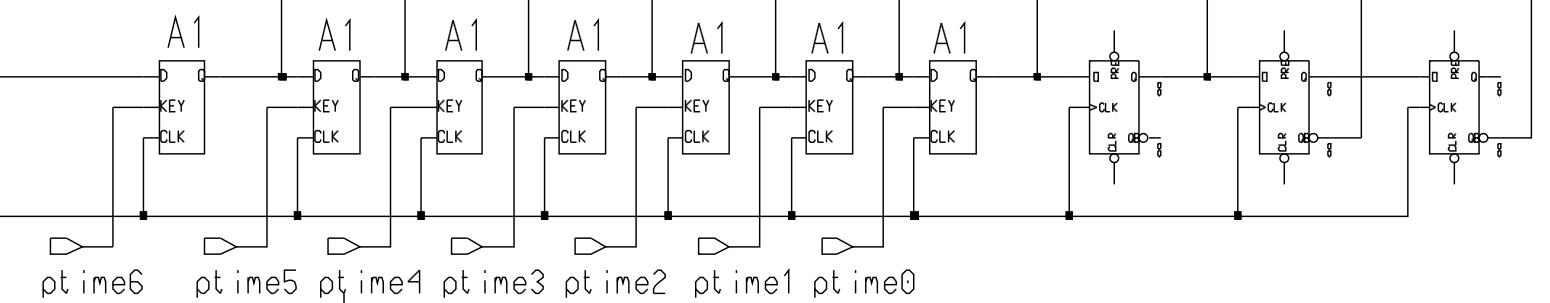
\includegraphics[keepaspectratio=true, width=0.9 \textwidth]{Images/peaking-time.png}
\caption{Comparator peaking time logic}
\label{img:peaking-time}
\end{figure}

The rightmost two flip-flops ensure that the signal has been below threshold for at least two clock cycles before trigger. This is designed to prevent retriggering on the same pulse.

The third flip-flop is a non-configurable requirement that N>th at the moment of the clock's rising edge.

The remaining flip-flops can be enabled to add a requirement that N be greater than threshold for additional clock cycles. Enabling one of the configurable flip-flops requires that it be over threshold for at least 25 ns before trigger. Enabling two flip flops requires that it be over threshold for at least 50 ns before trigger, and so on.

Disabling a flip-flop by asserting the KEY input effectively turns the flip-flop into a wire.

The 7 peak-time inputs are cleverly connected to the output package pins, so that we only require 3 pins to control the 7 input flip flops. This is because the order of the enabled flip-flops is irrelevant, it is only the total number of enabled flip-flops that we care about.

The signals on the front-end boards are expected to be around 150ns, and thus we would need 6 flip-flops to wait for the peak.

Overall, this logic is concisely summarized in Table~\ref{tab:pktime}.

\begin{table}[H]
\begin{center}
\begin{tabular}{ c   c   c }
\textbf{peaking\_{}time[2:0]} & \textbf{Flip-flops} & \textbf{Peaking Time (ns)} \\
\midrule
000 & 1 & 25 \\
001 & 2 & 50 \\
010 & 3 & 75 \\
011 & 4 & 100 \\
100 & 5 & 125 \\
101 & 6 & 150 \\
110 & 7 & 175 \\
111 & 8 & 200 \\
\end{tabular}
\end{center}
\caption{Comparator peaking-time logic}
\label{tab:pktime}
\end{table}


\subsection{Peaking Mode Inputs}\label{sec:pkmode}

An additional flexibility is implemented in the design, mainly for further fine tuning if it is required. This is implemented by the peaking mode bits.


There are two peaking mode bits, which according to best available documentation, provide the following effect:

\renewcommand{\arraystretch}{1.2}
\begin{table}[H]
\begin{center}
    \begin{tabular}{ c l }
        \textbf{peaking\_mode[1:0]} & \textbf{Peaking Mode} \\
        \midrule
        00 & Require TOT>THR for 1st Clock Only \\
        01 & Require TOT>THR for 1st+4th Clock  \\
        11 & Require TOT>THR for all 4 Clocks   \\
    \end{tabular}
\end{center}
\end{table}



Unfortunately it is unclear if or how this is accurate in the production version of the LCT-comparator chip. In reality, there are 7 pkmode inputs to the triad logic, but only 2 pkmode inputs on the comparator package.

\subsection{Packaging and Pinout}

%\begin {figure}
%\centering
%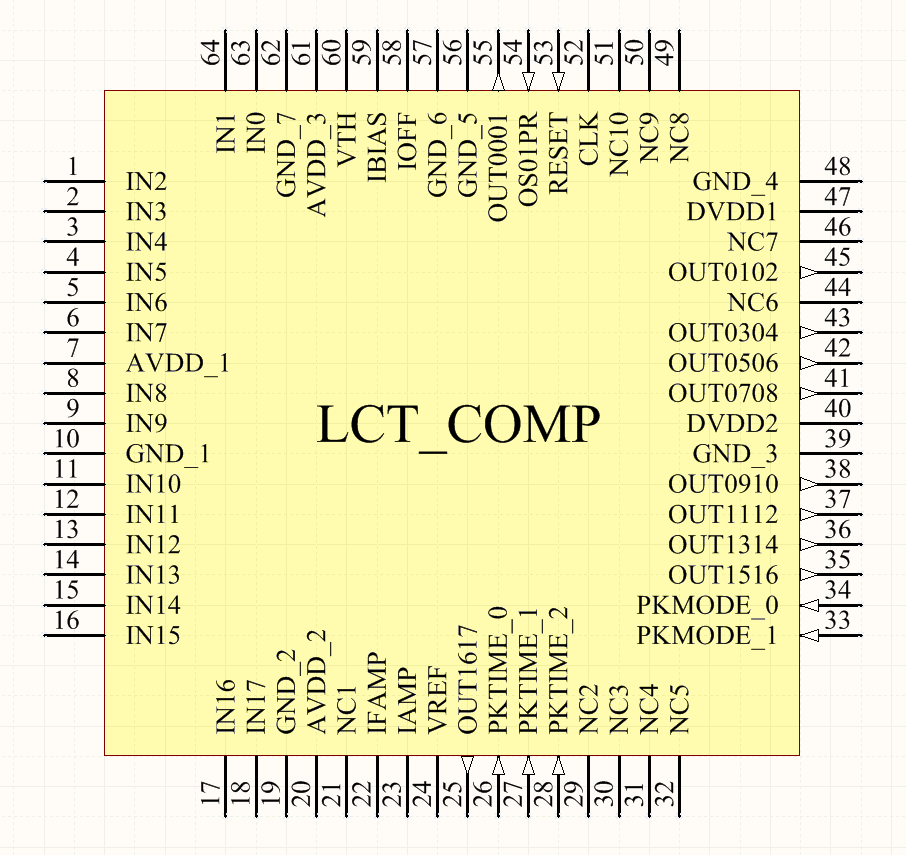
\includegraphics[keepaspectratio=true, width=5cm]{Images/chip_schematic.png}
%\caption {LCT Comparator Pinout}
%\end {figure}

%\scriptsize
\footnotesize
\begin{center}
\renewcommand{\arraystretch}{1.0}
\begin{tabular}{ | c | c | c | l | }

%%\begin{longtable}{ | c | c | c | p{10cm} | }
%%
%%\hline
%%\textbf{NAME} & \textbf{Type} & \textbf{PIN} & \textbf{DESCRIPTION}
%%\\\hline \endfirsthead \hline
%%\textbf{NAME} & \textbf{Type} & \textbf{PIN} & \textbf{DESCRIPTION}
%%\\\hline \endhead
%
%%\caption{Note that no current is sink or source from the logic Inputs, and logic Outputs are all buffered sustain a load of 20pF at 40MHz.}\\
%%\endlastfoot
%
%%\label{tab:pindescription}
%
%%\caption*{\large{\textbf{LCT Comparator Pin Description}}}


% BEGIN RECEIVE ORGTBL pinout
\hline
\textbf{NAME} & \textbf{TYPE} & \textbf{PIN} & \textbf{DESCRIPTION} \\
\hline
IN0 & In & 63 & Analog comparator inputs 0-18 \\
IN1 & In & 64 &  \\
IN2 & In & 1 &  \\
IN3 & In & 2 &  \\
IN4 & In & 3 &  \\
IN5 & In & 4 &  \\
IN6 & In & 5 &  \\
IN7 & In & 6 &  \\
IN8 & In & 7 &  \\
IN9 & In & 8 &  \\
IN10 & In & 9 &  \\
IN11 & In & 10 &  \\
IN12 & In & 11 &  \\
IN13 & In & 12 &  \\
IN14 & In & 13 &  \\
IN15 & In & 14 &  \\
IN16 & In & 15 &  \\
IN17 & In & 16 &  \\
IN18 & In & 17 &  \\
\hline
GND0 &  & 10 & Common ground to the entire chip \\
GND1 &  & 19 &  \\
GND2 &  & 39 &  \\
GND3 &  & 48 &  \\
GND4 &  & 62 &  \\
GND5 &  & 56 &  \\
GND6 &  & 57 &  \\
\hline
AVDD0 & In & 8 & +5V analog supply. \\
AVDD1 & In & 20 &  \\
AVDD1 & In & 61 &  \\
\hline
DVDD0 & In & 47 & +5V or +3.3V supply for the digital logic and 40MHz clock. \\
\hline
DVDD2 & In & 40 & +5V or +3.3V supply for the output buffers. \\
\hline
V$_{TH}$ & In & 60 & Threshold of the comparator array. \\
\hline
I$_{BIAS}$ & In & 59 & Bias current of 20 $\mu$A \\
I$_{OFF}$ & In & 58 & Bias current of 2 $\mu$A \\
I$_{FAMP}$ & In & 22 & Bias current of 10 $\mu$A \\
I$_{AMP}$ & In & 23 & Bias current of 80 $\mu$A \\
\hline
$V_{REF}$ & In & 24 & Analog reference voltage. \\
\hline
OUT$_{0102}$ & Out & 45 & Encoded half-strip trigger data. \\
OUT$_{0304}$ & Out & 43 &  \\
OUT$_{0506}$ & Out & 42 &  \\
OUT$_{0708}$ & Out & 41 &  \\
OUT$_{0910}$ & Out & 38 &  \\
OUT$_{1112}$ & Out & 37 &  \\
OUT$_{1314}$ & Out & 36 &  \\
OUT$_{1516}$ & Out & 35 &  \\
\hline
OUT$_{0001}$ & Out & 55 & Provides the result from the comparator $Q_{0}<Q_{1}$ \\
OUT$_{1617}$ & Out & 25 & Provides the comparator result of $Q_{17}>Q_{16}$ \\
\hline
OS01PR & In & 55 & Neighboring comparator input. \\
\hline
NC1 & NA & 21 & Do not connect. \\
NC2 & NA & 29 &  \\
NC3 & NA & 30 &  \\
NC4 & NA & 31 &  \\
NC5 & NA & 32 &  \\
NC6 & NA & 44 &  \\
NC7 & NA & 46 &  \\
NC8 & NA & 49 &  \\
NC9 & NA & 50 &  \\
NC10 & NA & 51 &  \\
\hline
PKMODE0 & In & 34 & Controls peaking mode logic (cf. \autoref{sec:pkmode}). \\
\hline
PKTIME0 & In & 26 & Controls peaking time logic (cf. \autoref{sec:pktime}). \\
PKTIME1 & In & 27 &  \\
PKTIME2 & In & 28 &  \\
\hline
% END RECEIVE ORGTBL pinout
\end{tabular}
%\end{longtable}
\end{center}
\normalsize


%\begin{comment}
%#+ORGTBL: SEND pinout orgtbl-to-latex-verbatim :splice t :raw t :no-escape t
%|---------------+---------------+--------------+------------------------------------------------------------|
%| \textbf{NAME} | \textbf{TYPE} | \textbf{PIN} | \textbf{DESCRIPTION}                                       |
%|---------------+---------------+--------------+------------------------------------------------------------|
%| IN0           | In            |           63 | Analog comparator inputs 0-18                              |
%| IN1           | In            |           64 |                                                            |
%| IN2           | In            |            1 |                                                            |
%| IN3           | In            |            2 |                                                            |
%| IN4           | In            |            3 |                                                            |
%| IN5           | In            |            4 |                                                            |
%| IN6           | In            |            5 |                                                            |
%| IN7           | In            |            6 |                                                            |
%| IN8           | In            |            7 |                                                            |
%| IN9           | In            |            8 |                                                            |
%| IN10          | In            |            9 |                                                            |
%| IN11          | In            |           10 |                                                            |
%| IN12          | In            |           11 |                                                            |
%| IN13          | In            |           12 |                                                            |
%| IN14          | In            |           13 |                                                            |
%| IN15          | In            |           14 |                                                            |
%| IN16          | In            |           15 |                                                            |
%| IN17          | In            |           16 |                                                            |
%| IN18          | In            |           17 |                                                            |
%|---------------+---------------+--------------+------------------------------------------------------------|
%| GND0          |               |           10 | Common ground to the entire chip                           |
%| GND1          |               |           19 |                                                            |
%| GND2          |               |           39 |                                                            |
%| GND3          |               |           48 |                                                            |
%| GND4          |               |           62 |                                                            |
%| GND5          |               |           56 |                                                            |
%| GND6          |               |           57 |                                                            |
%|---------------+---------------+--------------+------------------------------------------------------------|
%| AVDD0         | In            |            8 | +5V analog supply.                                         |
%| AVDD1         | In            |           20 |                                                            |
%| AVDD1         | In            |           61 |                                                            |
%|---------------+---------------+--------------+------------------------------------------------------------|
%| DVDD0         | In            |           47 | +5V or +3.3V supply for the digital logic and 40MHz clock. |
%|---------------+---------------+--------------+------------------------------------------------------------|
%| DVDD2         | In            |           40 | +5V or +3.3V supply for the output buffers.                |
%|---------------+---------------+--------------+------------------------------------------------------------|
%| V$_{TH}$      | In            |           60 | Threshold of the comparator array.                         |
%|---------------+---------------+--------------+------------------------------------------------------------|
%| I$_{BIAS}$    | In            |           59 | Bias current of 20 $\mu$A                                  |
%| I$_{OFF}$     | In            |           58 | Bias current of 2 $\mu$A                                   |
%| I$_{FAMP}$    | In            |           22 | Bias current of 10 $\mu$A                                  |
%| I$_{AMP}$     | In            |           23 | Bias current of 80 $\mu$A                                  |
%|---------------+---------------+--------------+------------------------------------------------------------|
%| $V_{REF}$     | In            |           24 | Analog reference voltage.                                  |
%|---------------+---------------+--------------+------------------------------------------------------------|
%| OUT$_{0102}$  | Out           |           45 | Encoded half-strip trigger data.                           |
%| OUT$_{0304}$  | Out           |           43 |                                                            |
%| OUT$_{0506}$  | Out           |           42 |                                                            |
%| OUT$_{0708}$  | Out           |           41 |                                                            |
%| OUT$_{0910}$  | Out           |           38 |                                                            |
%| OUT$_{1112}$  | Out           |           37 |                                                            |
%| OUT$_{1314}$  | Out           |           36 |                                                            |
%| OUT$_{1516}$  | Out           |           35 |                                                            |
%|---------------+---------------+--------------+------------------------------------------------------------|
%| OUT$_{0001}$  | Out           |           55 | Provides the result from the comparator $Q_{0}<Q_{1}$      |
%| OUT$_{1617}$  | Out           |           25 | Provides the comparator result of $Q_{17}>Q_{16}$          |
%|---------------+---------------+--------------+------------------------------------------------------------|
%| OS01PR        | In            |           55 | Neighboring comparator input.                              |
%|---------------+---------------+--------------+------------------------------------------------------------|
%| NC1           | NA            |           21 | Do not connect.                                            |
%| NC2           | NA            |           29 |                                                            |
%| NC3           | NA            |           30 |                                                            |
%| NC4           | NA            |           31 |                                                            |
%| NC5           | NA            |           32 |                                                            |
%| NC6           | NA            |           44 |                                                            |
%| NC7           | NA            |           46 |                                                            |
%| NC8           | NA            |           49 |                                                            |
%| NC9           | NA            |           50 |                                                            |
%| NC10          | NA            |           51 |                                                            |
%|---------------+---------------+--------------+------------------------------------------------------------|
%| PKMODE0       | In            |           34 | Controls peaking mode logic (cf. \autoref{sec:pkode}).     |
%|---------------+---------------+--------------+------------------------------------------------------------|
%| PKTIME0       | In            |           26 | Controls peaking time logic (cf. \autoref{sec:pktime}).    |
%| PKTIME1       | In            |           27 |                                                            |
%| PKTIME2       | In            |           28 |                                                            |
%|---------------+---------------+--------------+------------------------------------------------------------|
%
%#+TBLFM:
%\end{comment}

\section {Fabrication}

The fabrication of the LCT comparator chip was done in a 0.7 ${\mu}$m technology, developed by the Belgian firm Alcatel Mietec. The technology for this process has changed hands multiple times since its original development. First from Alcatel-Mietec, to AMI, then to the American firm ON-Semiconductor.

The design of the original chip was accomplished in two parts: (1) the analog comparator array, was designed and developed by J-C Santiard in the CERN electronics group, and (2) the digital portion of the chip, described in VHDL and implemented by automated process in the Alcatel-Mietec ASIC technology.  The combined chip, which incorporates both the custom analog amplifier/comparator array, and the digital logic, was created by Alcatel-Mietec. The IP for this chip, the hence the design (GDSII) files is in the hands of the fabricator---now ON-Semiconductor. As far as is known by us, these design files are not in anybody else's possession.  Fortunately, the GDSII files are all that is needed to produce a replicate mask set and fabricate additional LCT-Comparator chips.


\subsection{Packaging, die material, epoxy, etc.}

The package is a 64L TQFP with a body of 14 x 14 x 1.4 mm and a footprint of 14 x 14mm.

Encapsulation mold compound should have a very high resistivity. In 2000 fabrication, a conductive epoxy die attach was used. Jean-Claude's experience with the Gassiplex chip led him to prefer conductive epoxy die attach. The Gassiplex chip was a high input impedance analog chip, and it was found that the conductive epoxy resulted in better noise performance.

For the low impedance comparator inputs, however, it is believed that low-conductivity epoxy die attach will suffice.

For reference, 2000 fabrication used:
\begin{itemize}
    \item Die attach: 8361J
    \item Mold compound: EME-6650RA
    \item Die coat: Q3-6646
\end{itemize}

While 2015 fabrication used:
\begin{itemize}
    \item Die attach: CRM-1076WA
    \item Molding compound: EME-G631H
    \item No die coat possible
\end{itemize}

%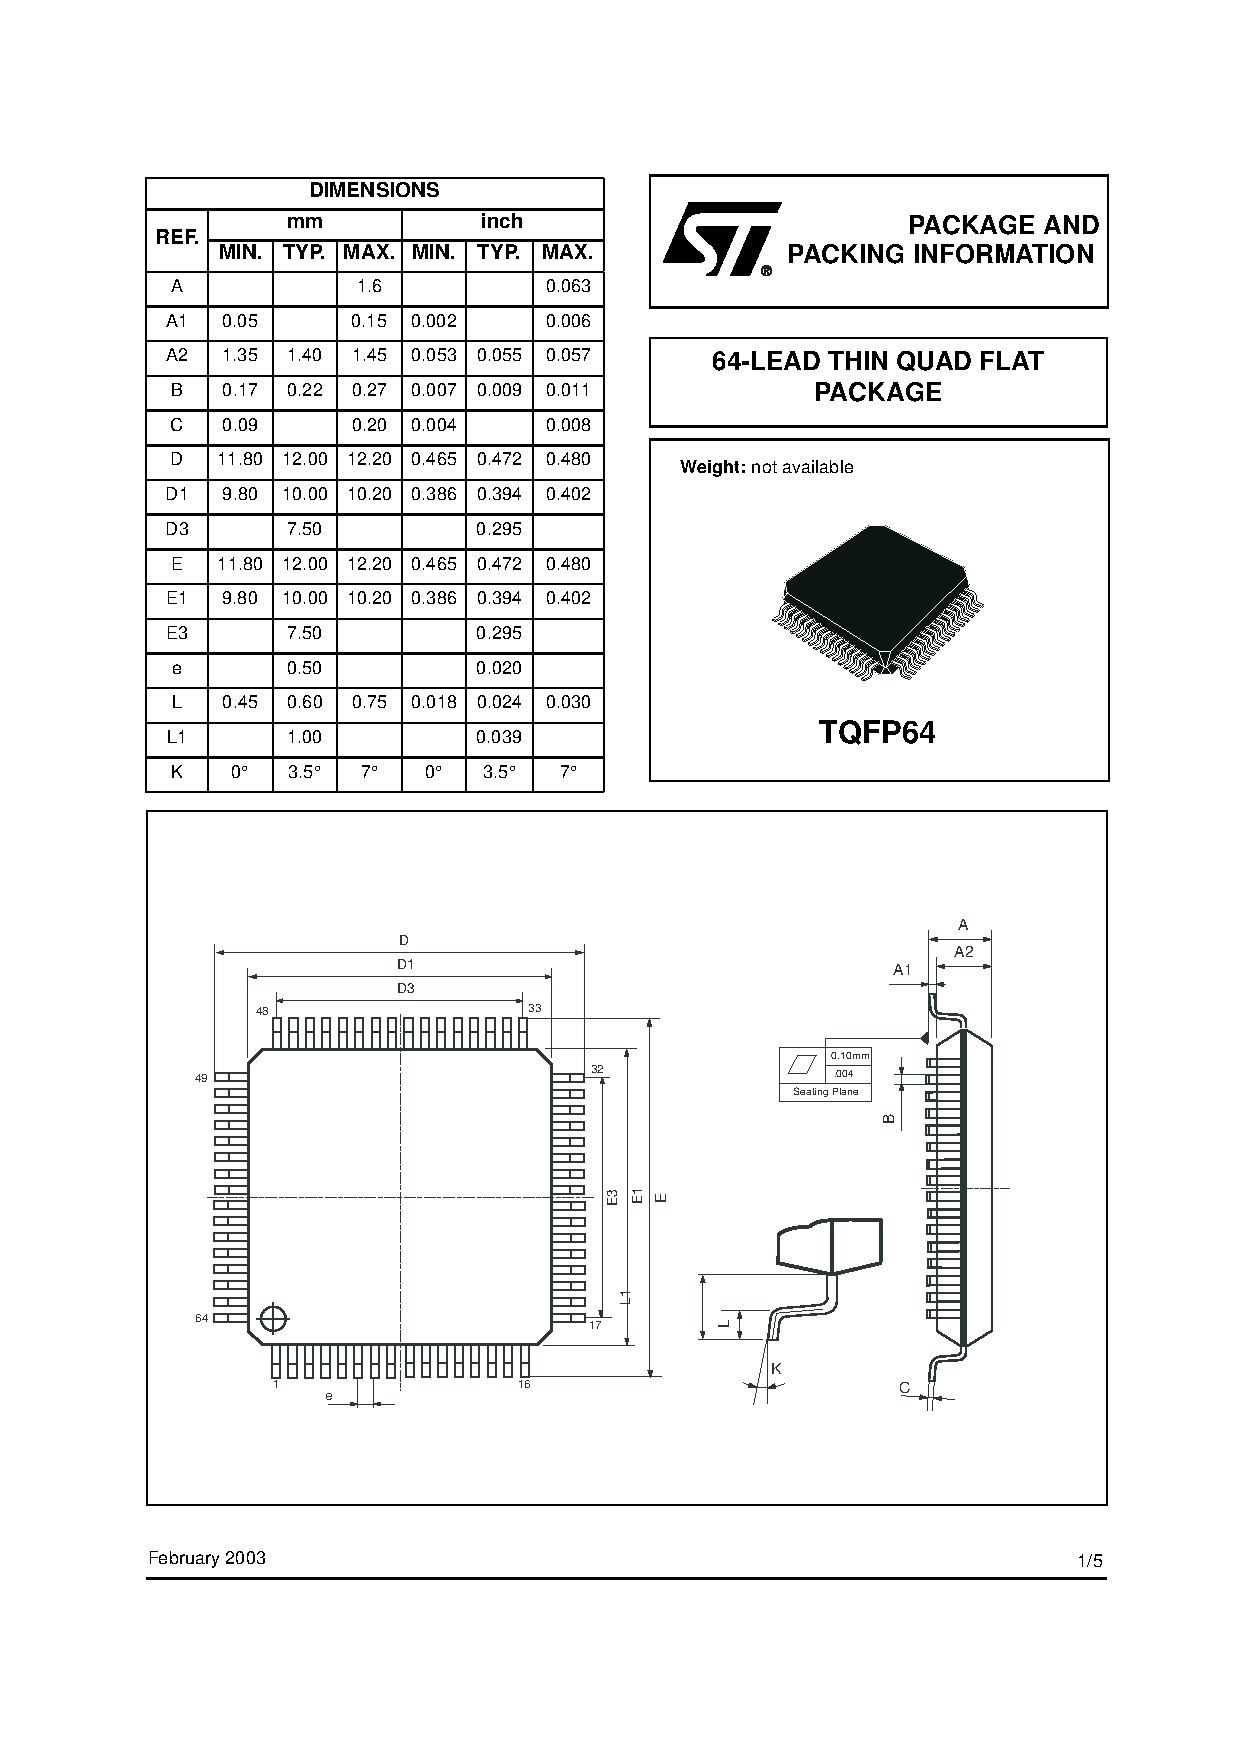
\includepdf[pages={1}]{Images/tqfp64.pdf}

%\begin {figure}
%\centering
%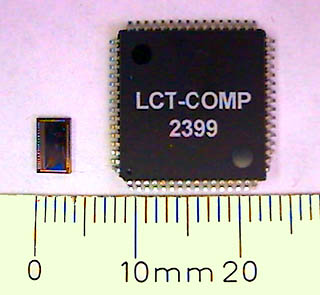
\includegraphics[keepaspectratio=true, width=0.4 \textwidth]{Images/new_asic_and_chip_sm.jpg}
%\caption {Unattached die (left) and packaged LCT Comparator (right)}
%\end {figure}

\subsection{Cost and Other Fabrication Information}

Full quotes from 2015 fabrication are included in Appendix \ref{appendix:fabricationquotes}.

A simple summary of the cost is as follows. The bulk of the cost occurs in non-recurring engineering, specifically, in the fabrication of a mask set and tooling for the encapsulation process. These NRE costs are

\begin{itemize}
    \item \$29417 for Mask set with 2 Wafers included
    \item \$4150 for tooling for encapsulation
\end{itemize}

Additional marginal costs are \$271 for encapsulation of each wafer (post sawing, yields 290 dies each), and \$2101 for each additional wafer. The total cost comes out to roughly \$40-50 per chip, depending on the percent yield.

Number of wafers needed will be yield dependent.

\begin{itemize}
    \item Yield = 80\% = 4 total wafers = \$38,885  (928 good chips) \\
          Yield = 65\% = 5 total wafers = \$41,228  (942 good chips) \\
          Yield = 55\% = 6 total wafers = \$43,601  (957 good chips) \\
          Yield = 45\% = 7 total wafers = \$45,974  (913 good chips)
\end{itemize}


Original yield was approximately 60\%. Should expect higher this time but we cannot be sure until testing.

Some key contact people at Imec who are familiar with the project are:

\begin{itemize}
\item Paul Malisse \\
Business Development Manager, imec IClink \\
Phone: +32 (0)16 281 272 \\
E-mail: \url{mailto:Paul.Malisse@imec.be}{Paul.Malisse@imec.be}

\item Carl Das, Director ASIC Services \\
Phone: +32 16 28 12 48 \\
Email: \url{mailto:Carl.Das@imec.be}{Carl.Das@imec.be}
\end{itemize}


%\newpage

\section{Testing}

\subsection{Test Descriptions}

\subsubsection{Thresholds and Offsets}

The testing of the LCT-COMPARATOR is based around providing pulses of programmable amplitude to neighboring half-strips and measuring the resulting digital response of the chip.

To begin with some definitions:

\begin{enumerate}

\item Thresholds:

The threshold is the amplitude of the central injected pulse such that the
comparator produces a response, on \textit{either} halfstrip of the central
strip. The threshold is set high enough that the L>R or R>L comparator offsets
are always exceeded, so we are measuring only the characteristics of the
N\_GT\_TH comparator (i.e. the OS01TH, OS02TH etc.).

In other words, we are checking the second bit of the comparator triad.

\item Offsets:

The offset is the difference in amplitude between the left and right
pulses at the minimum setting such that the comparator produces the
correct half-strip response.

In other words, we are checking the third bit of the comparator triad.

\end{enumerate}

The testing procedure is as follows:

\begin{enumerate}

\item The pulses should be multiplexed such that
%$(Q_{n} > Q_{n+1} > Q_{n-1})$.
We start with
%$n=1$,
so that IN1 receives a large pulse, IN2 receives a medium pulse, and IN0 receives a small pulse.  This would correspond to a hit on the right half strip of IN1.

%%TODO: what is this number
\item We test over a range of central amplitudes between 10 and 40 mV, in 2mV steps. At each voltage setting, we pulse the strips 100 times, keeping track of the triad response.  There will initially be no response at all from the triad logic (\texttt{000}).  At some point, a response will be seen, but which may or may not be on the right half-strip. That is, for Strip 1 we may see \texttt{100} (left hs) or \texttt{101} (right hs). The minimum setting when the triad output is \texttt{100} or \texttt{101} for at least 50\% of pulses, we record as the threshold.
%
%\item This is then repeated for with $n=2$, so that IN2 receives a large pulse, IN3 receives a medium pulse, and IN1 receives a small pulse.  This would correspond to a hit on the right half strip of IN2. And similarly for $n=3{\ldots}16$. This yields 16 threshold values, which we label as the Right>Left Thresholds.
%
%\item We then reduce the comparator threshold to 0mV, and configure the multiplexors in the same way. This time, we are looking to ensure that the triad output is on the correct half-strip that it has been configured for. At the minimum central pulse amplitude where the correct half-strip response is seen for at least 50\% of pulses, we take the difference between the right and left amplitudes $(V_{n+1} - V_{n-1})$, and call this the offset. Again, this yields 16 offsets values which we label as Right>Left Offsets.

%\item Now, we repeat this entire procedure with the opposite multiplexing configuration. Now, we want to have $Q_{n} > Q_{n-1} > Q_{n+1}$. We start with $n=1$, so that IN1 receives a large pulse, IN2 receives a small pulse, and IN0 receives a medium pulse.  This would correspond to a hit on the left half strip of IN1.

\item The same procedure is repeated, yielding 16 offsets and thresholds measurements, this time labeled as the Left>Right Thresholds and Offsets.

\end {enumerate}



\subsubsection{Additional Digital IO}

\begin{enumerate}

    \item OSO1PR (COMP\_IN)
    This input has to be tested during the test of the first channels (OUT0102). When applying on this input a logic signal of 300 ns width in phase with the input, the pattern 100 has to be canceled.

    \item OUT0001
    The OUT0001 pin is the comparator output of IN0/IN1. It is left unconnected on the (D)CFEB and does not need to be tested.

    \item OUT1617 (COMP\_OUT)
    OUT1617 is the comparator connected between IN16/IN17, which is connected to the next OSO1PR pin of the next (D)CFEB. The width of this output pulse is large enough to be detected at the 40 MHz clock.

    In the setting where the large central pulse is connected to IN16, and the medium pulse is connected to IN17 we should see

\end{enumerate}

\subsubsection {Supply Currents}

It is important to measure the current consumption of the LCT-Comparator chip, both in the digital and analog sections of the chip. The socketed design of tester boards makes direct temperature measurements difficult, but high temperature and high current will typically go hand-in-hand.

The current measurement can be as simple as passing all of the current to the chip through small value (e.g. 0.01 OHM) 1\% burden resistors. The voltage drop across the resistor can be amplified, and measured by ADC.

Any chips with high current consumption should be marked as NO GOOD.

\subsubsection{Bias Currents}

%The LCT-Comparator chip has three pins accepting bias currents: $I_{famp}$, $I_{amp}$, and $I_{off}$.
%
The nominal values of these currents are set simply by the external circuit that is powering them. A clean 5V analog supply should be connected, in series with a resistor, to each of these pins, and the bias current \emph{should} simply be given by $ V=IR $.
%
Any discrepancy in these currents would indicate something rather wrong in the analog amplifier/comparator network, and these chips should be rejected as NO GOOD.

\subsubsection{Peaking Time and Mode}

\begin {enumerate}

\item Peak Mode:

Peaking mode bits control the manner in which the triad logic finds a peak. Precise descriptions are given above.  It was found during the testing of the old comparator ASICs that changing of the peaking mode bits had little-to-no observable effect on the output. As such, this functionality was never tested during production, and should be OK to ignore.

\item Peak Time:

The peaking time bits are used to instantiate the size of the peaking bit shift-register. Again, see above for details.

By controlling the peaking-time bits, we are able to manipulate the LCT-Comparator's response to input pulses of varying width. With the peaking-time set to a large value, very short pulses will not illicit responses in the triad outputs.

In principle, the peaking time bits are straightforward to test. By sending large pulses (thus separate the influence of thresholds and offsets), and scanning over the phase space determined by all the combinations of peaking-time settings, and pulse widths, we can ensure that pulses are only seen at the settings in which they are expected.

\end{enumerate}


%
\subsection {Testing results}

In the original testing (circa 2000) by Santiard, a high speed 250MHz DAC module was used to directly synthesize a pulse of programmable shape and amplitude. This pulse was drove three attenuators, of 15 dB, 13 dB, and 6 dB, to generate Low, Medium, and High amplitude pulses, respectively. These three pulses feed into a bank of multiplexer chips, which are able to drive any one pulse to any one analog input of the comparator.

The testing is done on the basis of a GOOD or NO GOOD classification, with the limits of the specifications determined by measuring the characteristics (threshold, offsets, supply currents, bias currents) of a sampling of chips and producing cuts on the distribution. Any chips with a parameter outside of the range of tolerance will be classified as NO GOOD.

% \begin {figure}
% \centering
% 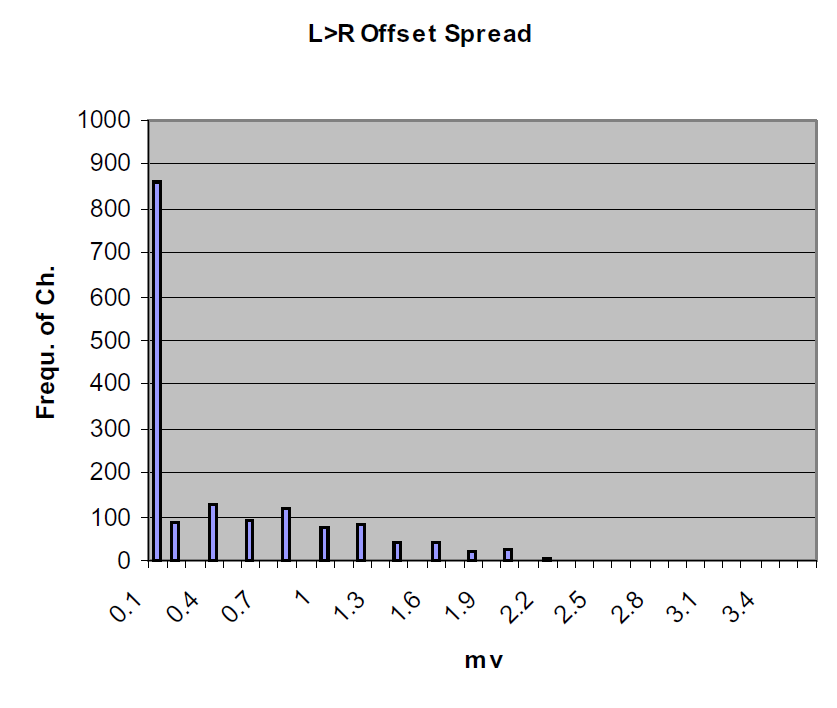
\includegraphics[keepaspectratio=true, width=0.75 \textwidth]{Images/l_gt_r_offsets.png}
% \caption {Left>Right Offsets Distribution from 2000 Testing.}
% \end {figure}%          %
%
% \begin {figure}
% \centering
% 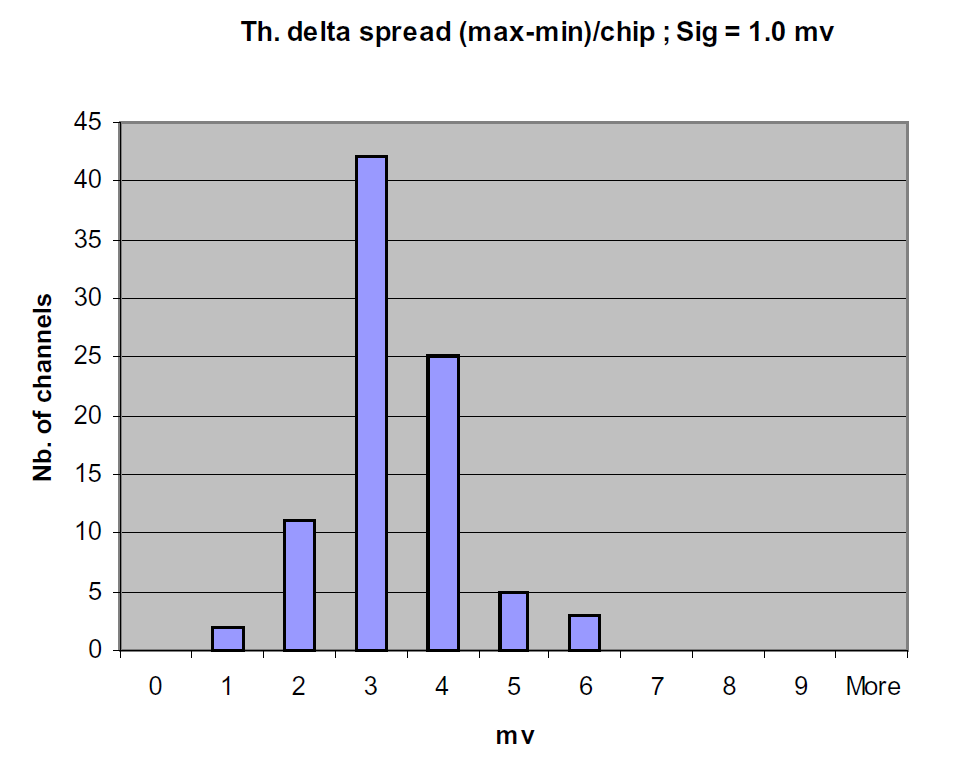
\includegraphics[keepaspectratio=true, width=0.75 \textwidth]{Images/thresholds_delta_spread.png}
% \caption {Thresholds Delta (Threshold Max-Min) Distribution from 2000 Testing.}
% \end {figure}%          %
%
% \begin {figure}
% \centering
% 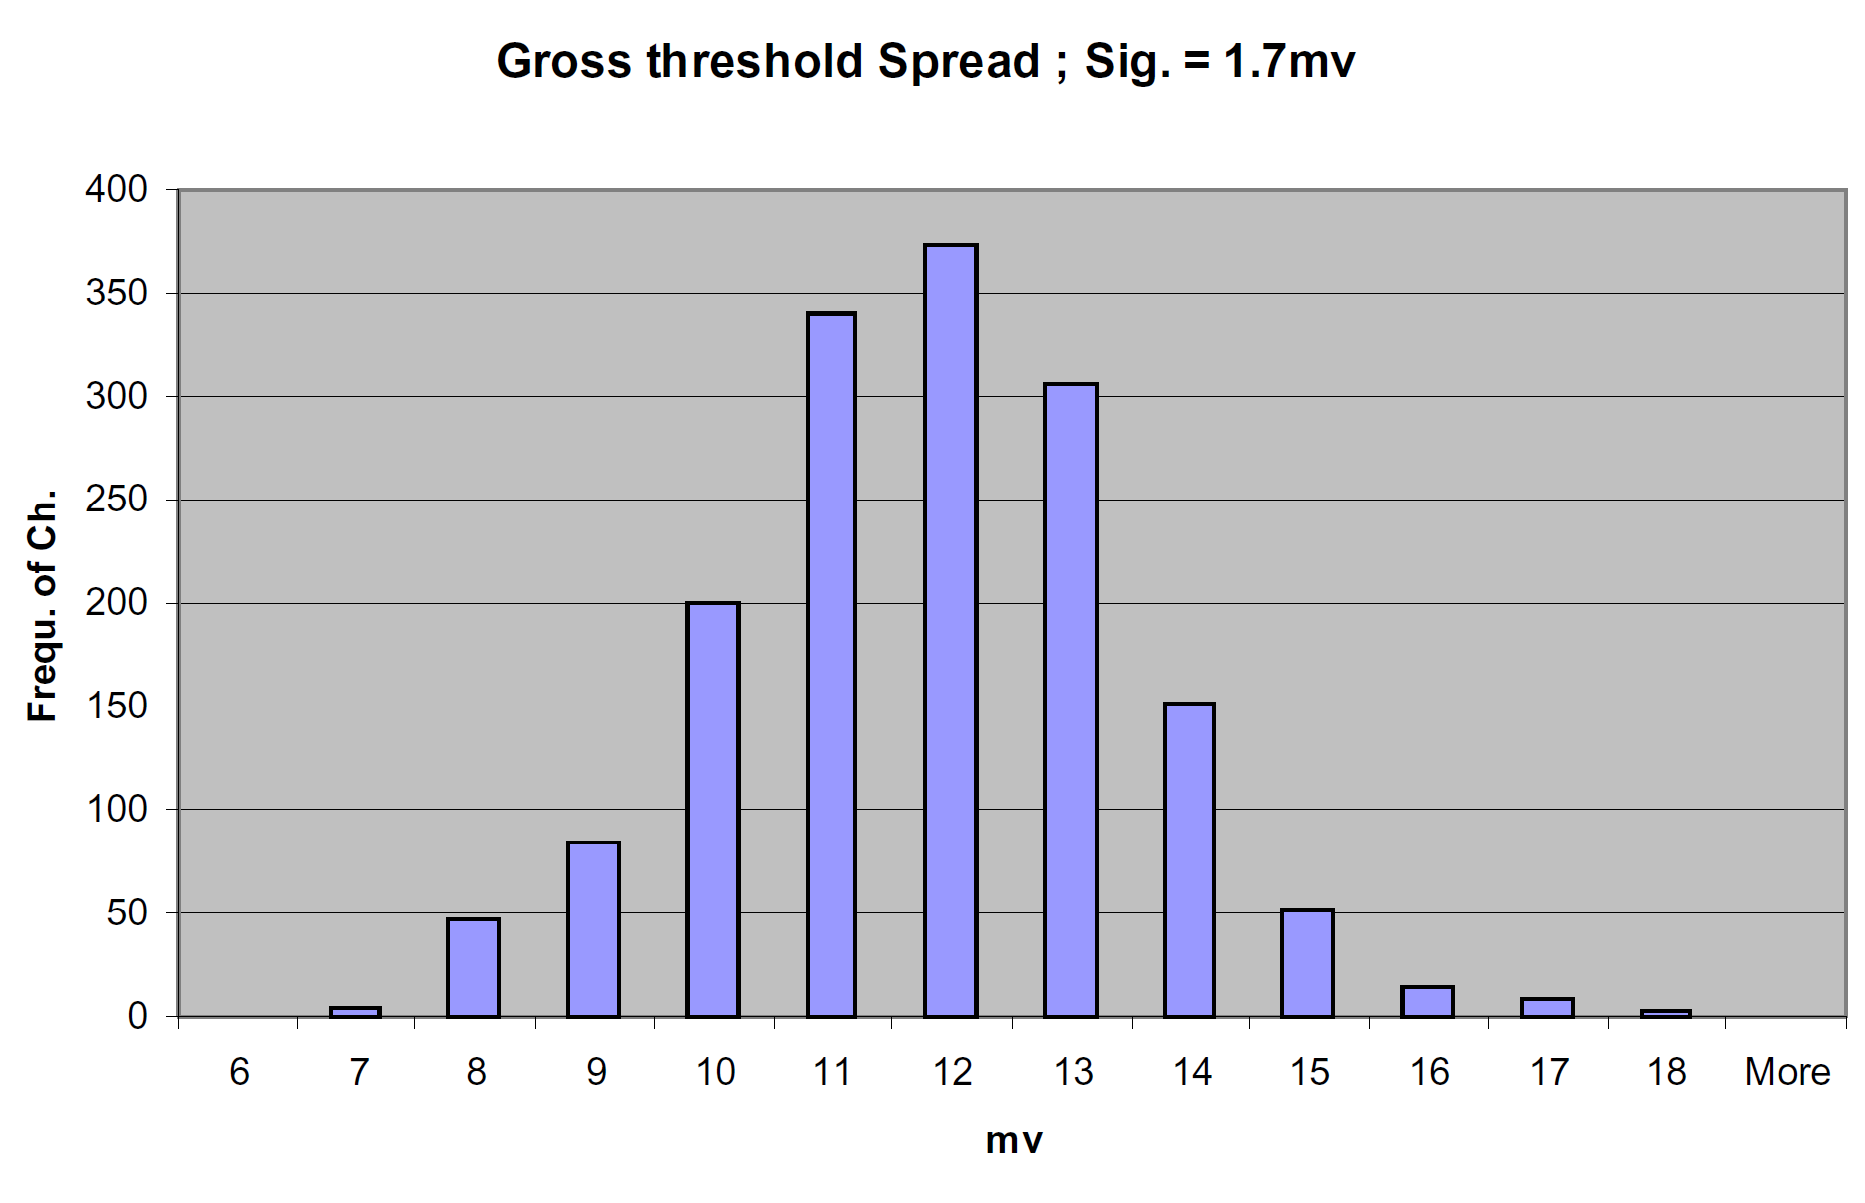
\includegraphics[keepaspectratio=true, width=0.75 \textwidth]{Images/thresholds.png}
% \caption {Gross Thresholds Distribution from 2000 Testing.}
% \end {figure}%          %

2015 testing follows a similar routine. A semi-Gaussian waveform is generated from a square wave of well-controlled amplitude, which is passed through a six-pole semi-Gaussian shaper (similar to the Buckeye shaping circuit that drives the LCT-Comparator). Three attenuators divide the signal, which is then fed into a bank of multiplexers. The testing methodology follows directly from the 2000 measurements.

"Another part to test is the peak-mode and the peak-time bits. During the thresholds and offsets measurements the peak-mode has to be 10 and the peak-time 100. The action of varying the value of peak-mode has no visible effect. Then it's not necessary to test it, only the connectivity. When varying the peak-time bits, the inputs-outputs delay will vary from 20ns (000) to 160ns (111) by steps of 20ns. Varying 3 times the 3 bits can test this features: 001, 010, and 100 on chanel one and with 50mV input.


\pagebreak


    % \subsection{LCT-COMP 2015 Test Board}
    %
    % \subsubsection{Test Procedure}
    %
    % \newpage %        \subsubsection{FPGA Control Registers} % %        The following table describes the FPGA control registers in the LCT-COMP 2015 Test Board. %        \begin{center} %            \renewcommand{\arraystretch}{1.4} %            \begin{longtable}{ | R{1cm} | C{0.75cm} | p{3 cm} | C{1.25 cm} | p{8cm} | } %            \endfirsthead %            %\hline %            %\textbf{Bit} & \textbf{Dir} & \textbf{Signal} & \textbf{Default} & \textbf{Description} \\\hline %        \endhead
    %
    % \endlastfoot
    %
    % \multicolumn{5}{l}{\textbf{Adr 0x01: ADR\_COMP\_CONFIG \hfill Comparator Configuration Register}} \\
    % \hline
    % \textbf{Bit} & \textbf{Dir} & \textbf{Signal} & \textbf{Default} & \textbf{Description} \\\hline
    % \nopagebreak
    % 0            & RW           & pktime0         & ?                & Peaking Time Bit 0 \\\hline
    % 1            & RW           & pktime1         & ?                & Peaking Time Bit 1 \\\hline
    % 2            & RW           & pktime2         & ?                & Peaking Time Bit 2 \\\hline
    % 3            & RW           & pkmode0         & ?                & Peaking Mode Bit 0 \\\hline
    % 4            & RW           & pkmode1         & ?                & Peaking Mode Bit 1 \\\hline
    % 5            & RW           & lctrst          & 0                & LCT Reset \\\hline
    % 6            & RW           & /cdac\_en       & 1                & Comparator Threshold DAC /Enable  \\\hline
    % 7            & RW           & cdac\_din       & 0                & Comparator Threshold DAC Serial Data Input \\\hline
    % 8            & RW           & cdac\_ck        & 0                & Comparator Threshold DAC Serial Data Clock \\\hline
    % 31:9         &              & Unassigned      &                  & \\\hline
    %
    % \multicolumn{5}{l}{\textbf{Adr 0x02: ADR\_PULSE\_CTRL \hfill Pulse Control Register}} \\
    %
    % \hline
    % \textbf{Bit} & \textbf{Dir} & \textbf{Signal}         & \textbf{Default} & \textbf{Description} \\\hline
    % \nopagebreak
    % 0            & RW           & fire\_pulse             & 0                & Rising edge inject a single pulse (if pulser\_ready)\\\hline
    % 4:1          & RW           & pulse\_width[3:0]       & 0                & Integer digi pulse width (in 25ns clock cycles) \\\hline
    % 5            & RW           & /pulsedac\_en           & 0                & Pulse DAC /Enable \\\hline
    % 6            & RW           & pulsedac\_din           & 0                & Pulse DAC Serial Data In\\\hline
    % 7            & RW           & pulsedac\_sclk          & 0                & Pulse DAC Serial Data Clock\\\hline
    % 8            & RW           & halfstrips\_errcnt\_rst & 0                & Rising edge resets halfstrips error counter\\\hline
    % 9            & RW           & compout\_errcnt\_rst    & 0                & Rising edge resets COMPOUT error counter\\\hline
    % 10           & RW           & compin\_inject          & X                & Determines whether pulse injector will inject COMPIN during pulsing\\\hline
    % 13:11        & RW           & bx\_delay[3:0]          & X                & Integer bx (25 ns) delay after pulse injection, before reading out strips \\\hline
    % 14           & RW           & compout\_expect         & X                & Set expected comparator COMPOUT output \\\hline
    % 18:15        & RW           & triad\_persist[3:0]     & 0                & Set Triad State-machine persist \\\hline
    % 19           & RW           & triad\_persist1         & 1                & Set Triad State-machine persist1 \\\hline
    % 20           & RW           & thresholds\_errcnt\_rst & 0                & Rising edge resets thresholds error counter \\\hline
    % 31:21        &              & Unassigned              &                  & \\\hline
    %
    %
    % \multicolumn{5}{l}{\textbf{Adr 0x03: ADR\_MUX1 \hfill Mux Control Bank 1}} \\\hline
    % \nopagebreak
    % \textbf{Bit} & \textbf{Dir} & \textbf{Signal} & \textbf{Default} & \textbf{Description} \\\hline
    % 0            & RW           & mux\_a0\_prev   & 0                & IN00 Mux Control Bit 0  \\\hline
    % 1            & RW           & mux\_a1\_prev   & 0                & IN00 Mux Control Bit 1  \\\hline
    % 2            & RW           & mux\_a0\_next   & 0                & IN17 Mux Control Bit 0  \\\hline
    % 3            & RW           & mux\_a1\_next   & 0                & IN17 Mux Control Bit 1  \\\hline
    % 31:4         &              & Unassigned      &                  & \\\hline
    %
    %
    % \pagebreak
    % \multicolumn{5}{l}{\textbf{Adr 0x04: ADR\_MUX2 \hfill Mux Control Bank 2}} \\\hline
    % \textbf{Bit} & \textbf{Dir} & \textbf{Signal} & \textbf{Default} & \textbf{Description} \\\hline
    % 0            & RW           & mux\_a0\_0      & 0                & IN01 Mux Control Bit 0  \\\hline
    % 1            & RW           & mux\_a1\_0      & 0                & IN01 Mux Control Bit 1  \\\hline
    % 2            & RW           & mux\_a0\_1      & 0                & IN02 Mux Control Bit 0  \\\hline
    % 3            & RW           & mux\_a1\_1      & 0                & IN02 Mux Control Bit 1  \\\hline
    % 5            & RW           & mux\_a1\_2      & 0                & IN03 Mux Control Bit 1  \\\hline
    % 6            & RW           & mux\_a0\_3      & 0                & IN04 Mux Control Bit 0  \\\hline
    % 7            & RW           & mux\_a1\_3      & 0                & IN04 Mux Control Bit 1  \\\hline
    % 8            & RW           & mux\_a0\_4      & 0                & IN05 Mux Control Bit 0  \\\hline
    % 9            & RW           & mux\_a1\_4      & 0                & IN05 Mux Control Bit 1  \\\hline
    % 10           & RW           & mux\_a0\_5      & 0                & IN06 Mux Control Bit 0  \\\hline
    % 11           & RW           & mux\_a1\_5      & 0                & IN06 Mux Control Bit 1  \\\hline
    % 12           & RW           & mux\_a0\_6      & 0                & IN07 Mux Control Bit 0  \\\hline
    % 13           & RW           & mux\_a1\_6      & 0                & IN07 Mux Control Bit 1  \\\hline
    % 14           & RW           & mux\_a0\_7      & 0                & IN08 Mux Control Bit 0  \\\hline
    % 15           & RW           & mux\_a1\_7      & 0                & IN08 Mux Control Bit 1  \\\hline
    % 16           & RW           & mux\_a0\_8      & 0                & IN09 Mux Control Bit 0  \\\hline
    % 17           & RW           & mux\_a1\_8      & 0                & IN09 Mux Control Bit 1  \\\hline
    % 18           & RW           & mux\_a0\_9      & 0                & IN10 Mux Control Bit 0  \\\hline
    % 19           & RW           & mux\_a1\_9      & 0                & IN10 Mux Control Bit 1  \\\hline
    % 20           & RW           & mux\_a0\_10     & 0                & IN11 Mux Control Bit 0  \\\hline
    % 21           & RW           & mux\_a1\_10     & 0                & IN11 Mux Control Bit 1  \\\hline
    % 22           & RW           & mux\_a0\_11     & 0                & IN12 Mux Control Bit 0  \\\hline
    % 23           & RW           & mux\_a1\_11     & 0                & IN12 Mux Control Bit 1  \\\hline
    % 24           & RW           & mux\_a0\_12     & 0                & IN13 Mux Control Bit 0  \\\hline
    % 25           & RW           & mux\_a1\_12     & 0                & IN13 Mux Control Bit 1  \\\hline
    % 26           & RW           & mux\_a0\_13     & 0                & IN14 Mux Control Bit 0  \\\hline
    % 27           & RW           & mux\_a1\_13     & 0                & IN14 Mux Control Bit 1  \\\hline
    % 28           & RW           & mux\_a0\_14     & 0                & IN15 Mux Control Bit 0  \\\hline
    % 29           & RW           & mux\_a1\_14     & 0                & IN15 Mux Control Bit 1  \\\hline
    % 30           & RW           & mux\_a0\_15     & 0                & IN16 Mux Control Bit 0  \\\hline
    % 31           & RW           & mux\_a1\_15     & 0                & IN16 Mux Control Bit 1  \\\hline
    % \pagebreak
    %
    % \multicolumn{5}{l}{\textbf{Adr 0x05: ADR\_HALFSTRISP \hfill Decoded Halfstrip Hit Map}} \\\hline
    % \nopagebreak
    % \textbf{Bit} & \textbf{Dir} & \textbf{Signal} & \textbf{Default} & \textbf{Description} \\\hline
    % 0-31         & R            & halfstrips[31:0] & 0                & One-to-one mapping of hits on halfstrips 0--31\\\hline
    %
    % \multicolumn{5}{l}{\textbf{Adr 0x06: ADR\_ADC \hfill ADC Control/Readout}} \\\hline
    % \nopagebreak
    % \textbf{Bit} & \textbf{Dir} & \textbf{Signal} & \textbf{Default} & \textbf{Description} \\\hline
    % 0            & RW           & /adc\_cs         & 1                & ADC /Chip Select\\\hline
    % 1            & RW           & adc\_mosi        & 0                & ADC Serial Data In\\\hline
    % 2            & RW           & adc\_sclock      & 0                & ADC Serial Clock \\\hline
    % 3            & R            & adc\_miso        & 0                & ADC Serial Data Out \\\hline
    % 31:4         &              & Unassigned      &                  & \\\hline
    %
    % \multicolumn{5}{l}{\textbf{Adr 0x07: ADR\_DDD \hfill Comparator Clock Delay Control}} \\\hline
    % \nopagebreak
    % \textbf{Bit} & \textbf{Dir} & \textbf{Signal}  & \textbf{Default} & \textbf{Description} \\\hline
    % 0            & RW           & /ddd\_adr\_latch & 1                & DDD /Latch Address Pin\\\hline
    % 1            & RW           & ddd\_mosi        & 0                & DDD Serial Data In\\\hline
    % 2            & RW           & ddd\_sclock      & 0                & DDD Serial Clock \\\hline
    % 31:3         &              & Unassigned       &                  & \\\hline
    %
    %
    %
    % \end{longtable}
    % \end{center}

    \appendix
    \nosection{LCT-Comparator 2015 Fabrication Quotes}
    \label{appendix:fabricationquotes}
    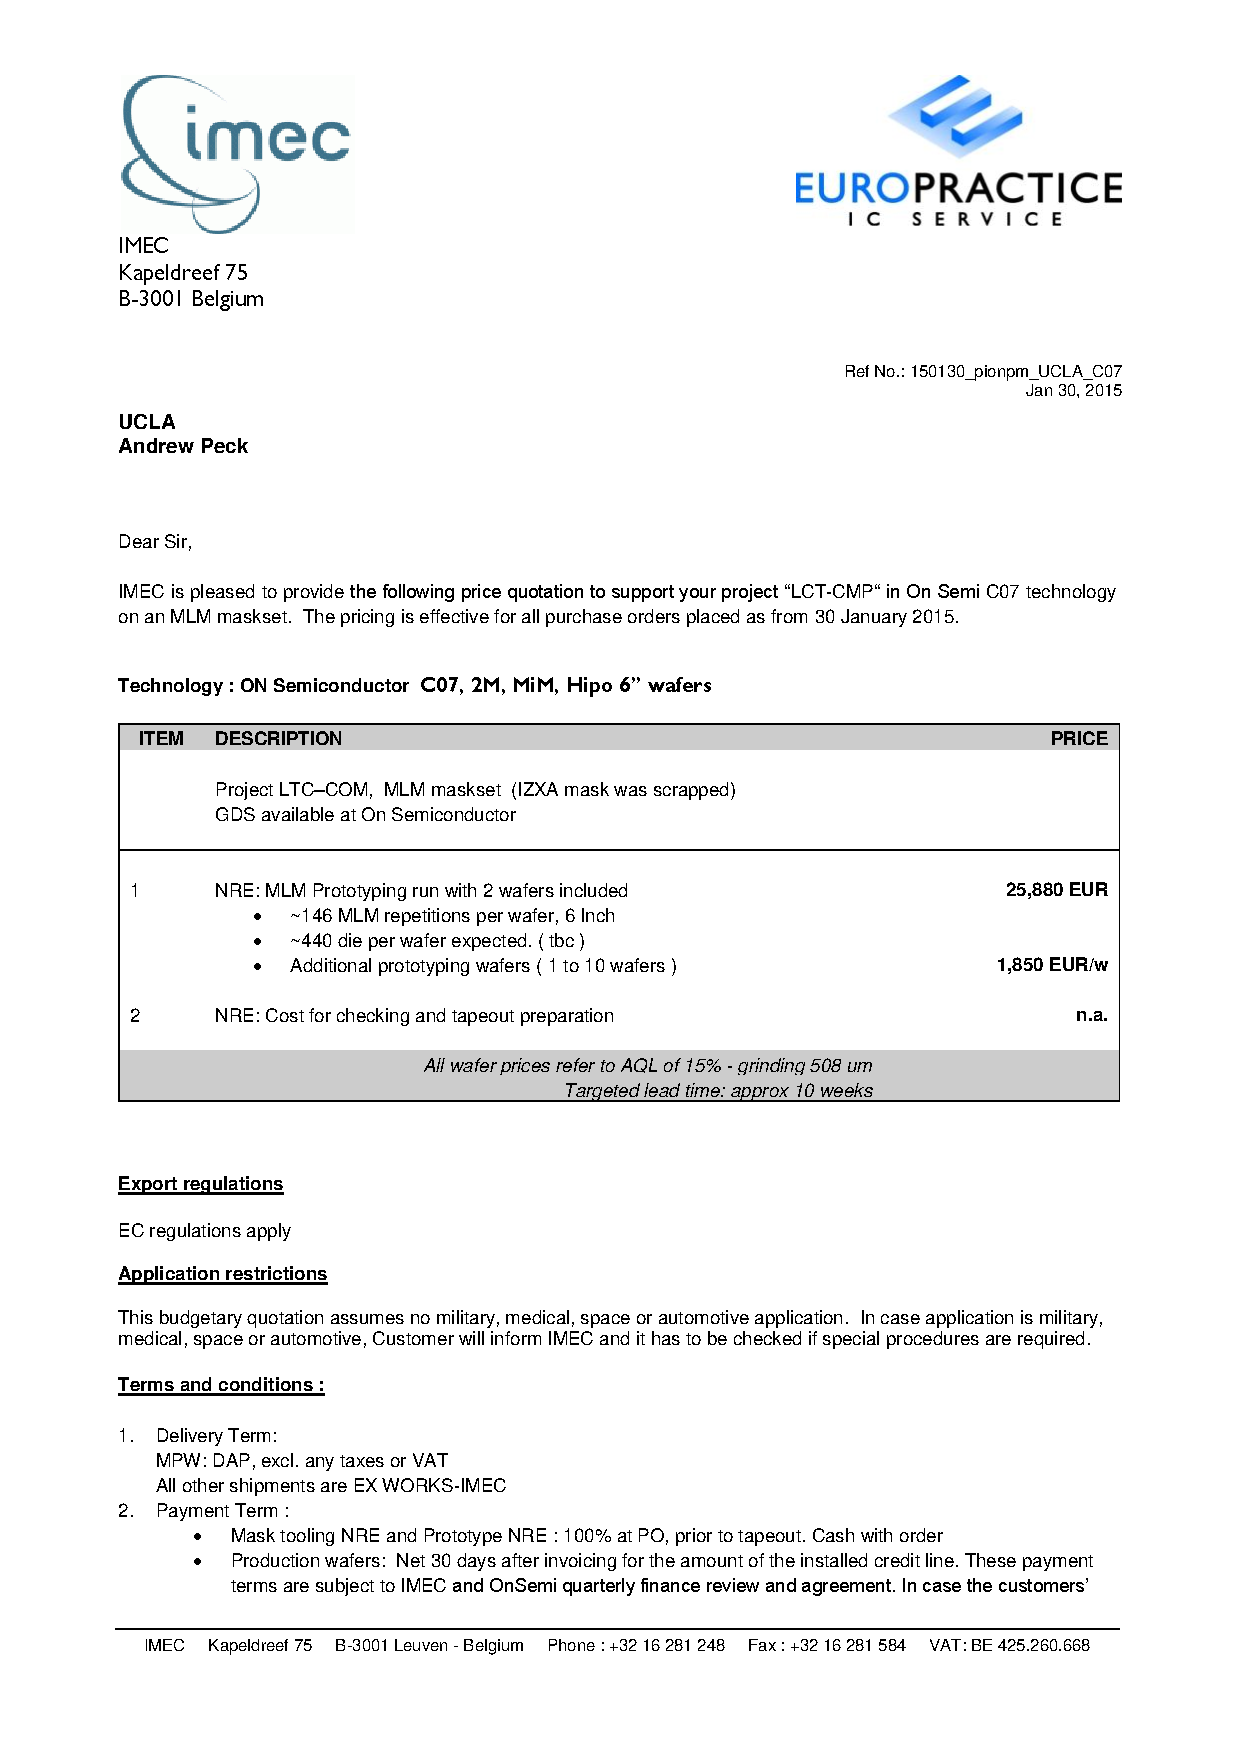
\includepdf[pages={1-2}]{Images/150130_pionpm_UCLA_C07.pdf}
    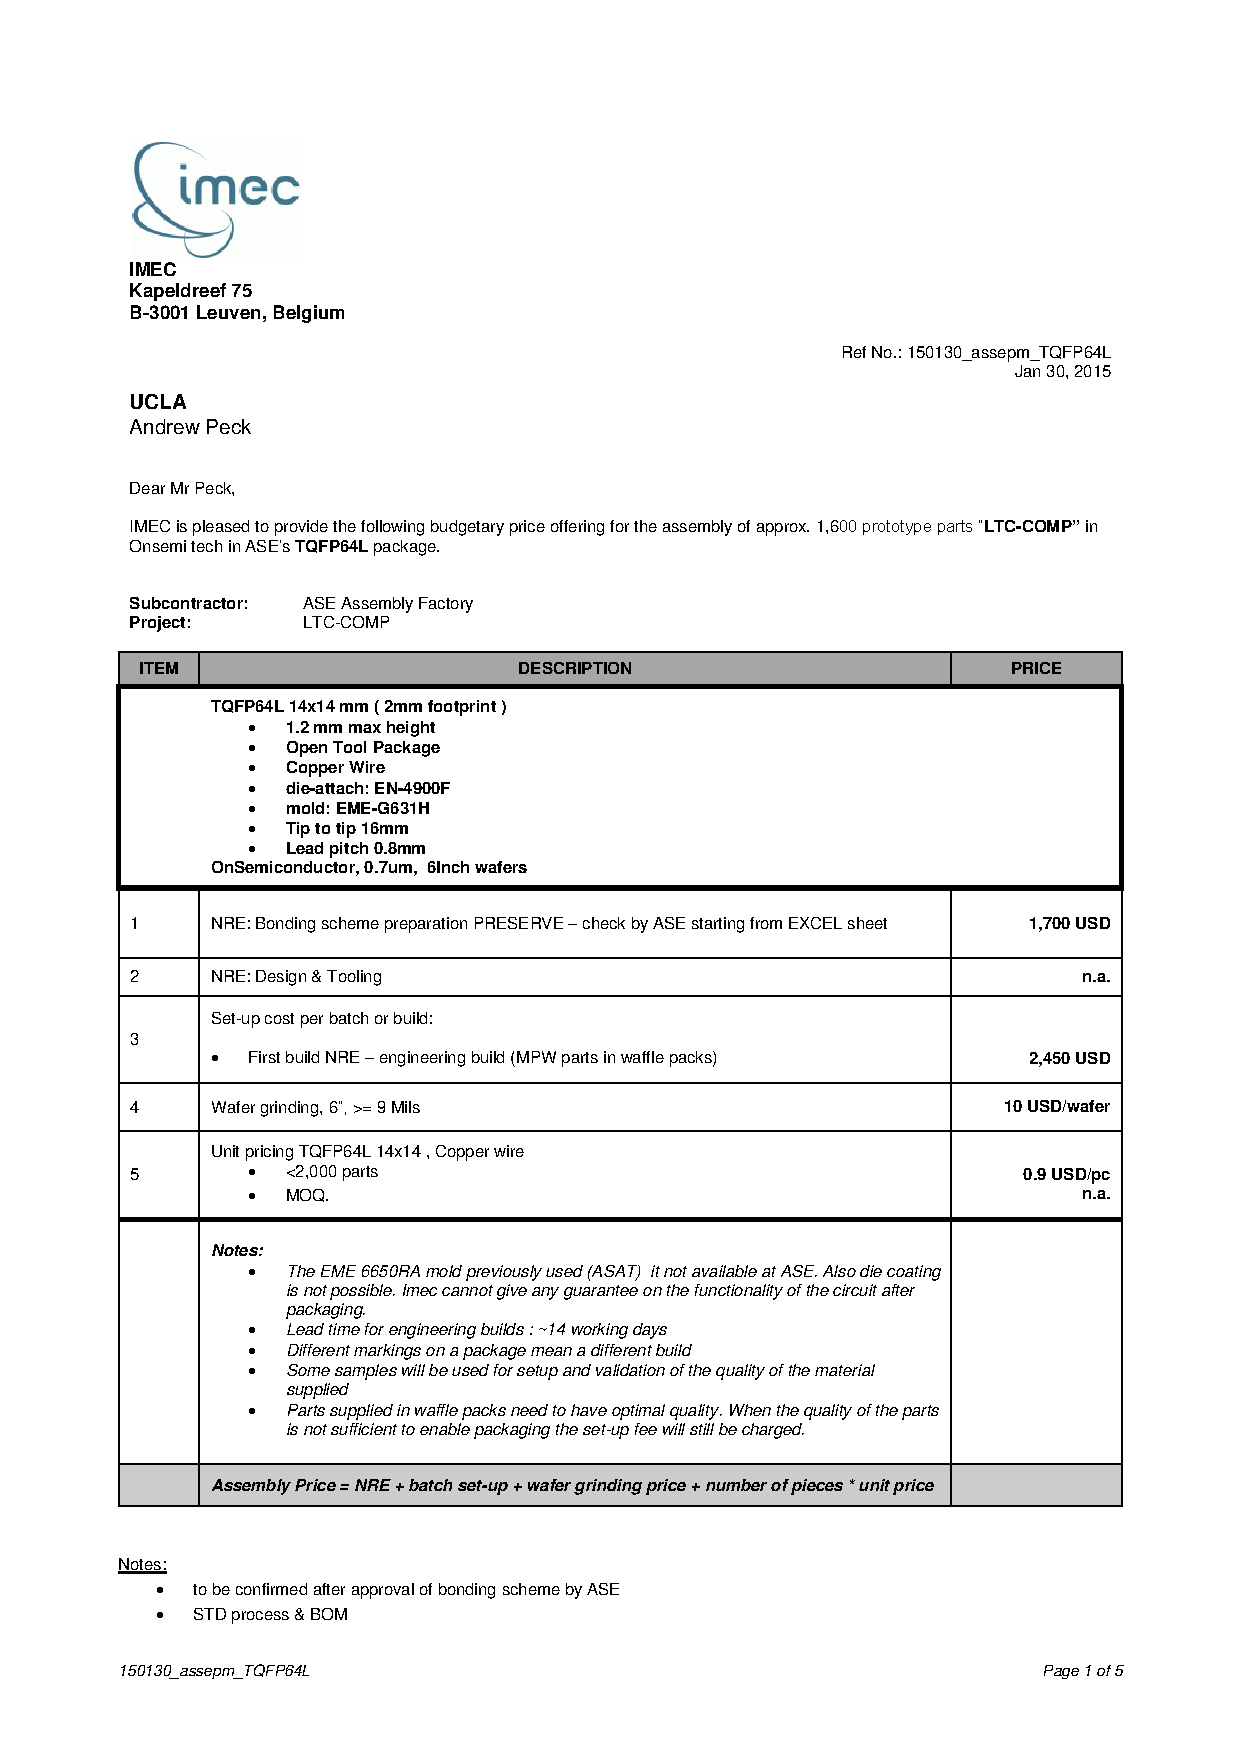
\includepdf[pages={1-2}]{Images/150130_assepm_TQFP64L.pdf}

\section {Schematics}

\end{document}


%%% Local Variables:
%%% mode: latex
%%% TeX-PDF-mode: t
%%% End:
